\documentclass[aip,cha,reprint,amsmath,amssymb,final]{revtex4-2}
\usepackage{graphicx}
\graphicspath{{figures/}{./}}
\usepackage{xurl}

\hyphenpenalty=10000
\exhyphenpenalty=10000
\tolerance=2000
\emergencystretch=1em

\begin{document}

\title{The Dynamic Existence Threshold: Organizational Consciousness across Complex Systems}
\author{Nathan M. Thornhill}
\affiliation{Independent Researcher\\
Fort Wayne, Indiana, USA\\
\texttt{research@nathanthornhill.com} $|$ \url{https://nathanthornhill.com}}

\begin{abstract}
Complex systems across disparate substrates share a common failure mode: the breakdown of balance between integration and differentiation. This paper introduces the Dynamic Existence Threshold (DET), a framework in which system state is characterized by two measurable quantities---integration ($I$), capturing coordinated multi-component coupling, and differentiation ($D$), capturing divergence from uniformity. The $I$--$D$ plane admits four theoretical states---dormant/fragmented (low $I$, high $D$), organized complexity (high $I$, high $D$), pathological cascade (high $I$, low $D$), and system death (low $I$, low $D$)---of which the present proxy metrics access primarily the dormant-to-cascade axis. Healthy baseline function corresponds to moderate values of both $I$ and $D$ at the center of this axis. The DET predicts that critical events correspond to exits from the $I$--$D$ balance zone and that approach to such exits produces measurable early warning signals. These predictions are tested across three domains---financial markets (6,785 trading days, 26 cascade events), space weather (9,802 days, 51 storm days), and human EEG (50 subjects, 57,212 epochs, Wake vs.\ N3 deep sleep)---using a five-layer measurement architecture with zero-parameter tuning between domains. Five tests confirm the framework: (1) events cluster at $I$--$D$ extremes; (2) events exit the balance zone faster than normal state changes ($p = 0.0001$); (3) rising variance of $|I - D|$ provides early warning 5--30 days before financial events and 5--10 days before space weather events (2.0$\times$ elevation, $p < 0.001$); (4) exit velocity discriminates events from normal with area under the curve (AUC) 0.692--0.843; and (5) in EEG, simple summation anti-predicts brain state (AUC 0.416) while the coupling metric $R \times S$ achieves AUC 0.909 (95\% CI [0.904, 0.913]), demonstrating that the framework captures multi-scale coordination rather than mere magnitude.
\end{abstract}
\maketitle

\section{Introduction}

When financial markets crash, geomagnetic storms erupt, or the brain descends into deep sleep, the underlying systems shift into qualitatively different states. Despite vast differences in substrate, these transitions share a structural signature: the breakdown of balance between how tightly a system's components are coupled (integration) and how distinctly they behave (differentiation). This paper introduces a measurable coordinate system---the integration-differentiation ($I$--$D$) plane---in which critical transitions across all three domains appear as departures from a common balance zone. Using identical metrics with no tuning between domains, we show that approaching these departures produces early warning signals consistent with critical slowing down, and that the framework captures structural coordination rather than mere signal magnitude---demonstrated by the finding that simple summation of neural frequency bands anti-predicts brain state while the structural coupling metric achieves 91\% classification accuracy.

A persistent question in complexity science is whether disparate systems---brains, markets, magnetospheres---undergo critical transitions through shared mechanisms or through substrate-specific processes that merely resemble one another superficially. The critical transitions literature has established that rising variance and autocorrelation precede tipping points across ecological, climatic, and financial systems~\cite{scheffer2009,dakos2012}, but these indicators describe \emph{symptoms} of approaching transitions without specifying the \emph{coordinate system} in which the transition occurs.

Integrated Information Theory (IIT) introduced the quantity $\Phi$ to characterize the degree to which a system is ``more than the sum of its parts''~\cite{tononi2016,tononi2004}. While IIT was developed primarily as a theory of consciousness, its core insight---that integration and differentiation jointly characterize system complexity---has implications far beyond neuroscience. Global Workspace Theory similarly emphasizes the interplay between distributed processing and unified access~\cite{baars1988}. Causal density, defined as the fraction of causally significant interactions in a network, has been proposed as a measure of dynamical complexity that peaks when integration and differentiation are jointly high~\cite{seth2011}.

The present work synthesizes these threads. IIT's $\Phi$ remains intractable for large-scale systems, and critical slowing down indicators, while powerful, describe symptoms without specifying the coordinate system in which transitions occur. Partial information decomposition (PID) has further revealed that synergistic and redundant information components respond asymmetrically to system perturbation~\cite{williams2010,popiel2020}, suggesting that coordination and overlap play distinct roles in system stability. The present paper proposes a dynamic framework grounded in these insights: systems do not merely need positive integrated information to persist---they must maintain balance between integration and differentiation over time.

The central hypothesis is straightforward. Integration ($I$) measures the degree of coordinated coupling among system components. Differentiation ($D$) measures the degree to which the system's activity profile diverges from uniformity. These two quantities define a phase space with four canonical states (Fig.~\ref{fig:quadrant}):

\begin{table}[!htbp]
\caption[Four-state model of the integration-differentiation phase space with states, I and D levels, and interpretations]{Four-state model of the $I$--$D$ phase space.}
\begin{ruledtabular}
\begin{tabular}{p{2.8cm}ccp{3.0cm}}
State & $I$ & $D$ & Interpretation \\
Dormant/fragmented & Low & High & Single component dominates \\
Organized complexity & High & High & Coordinated, differentiated activity \\
Cascade/seizure/crash & High & Low & Pathological synchronization \\
Death/off & Low & Low & System inactive \\
\end{tabular}
\end{ruledtabular}
\end{table}

The four states represent a theoretical taxonomy of the $I$--$D$ plane. Because the chosen proxy metrics are entropy-coupled (Section~3.6.4), empirical observations are largely constrained to the CASCADE--RECOVERY axis (high-$I$/low-$D$ to low-$I$/high-$D$). The Organized complexity and Death/off quadrants would require entropy-decoupled metrics---such as network-topology measures or formal partial information decomposition---to access reliably. The taxonomy remains useful as a conceptual map even when the accessible region is a subset of the full plane.

\emph{Note:} Empirically, healthy baseline function (wakefulness, normal markets) corresponds to moderate values of both $I$ and $D$---the center of the entropy axis---not to any single quadrant corner. The Dormant/fragmented and Cascade quadrants represent the two extremes of this axis, with healthy function between them.

\begin{figure*}[t]
\centering
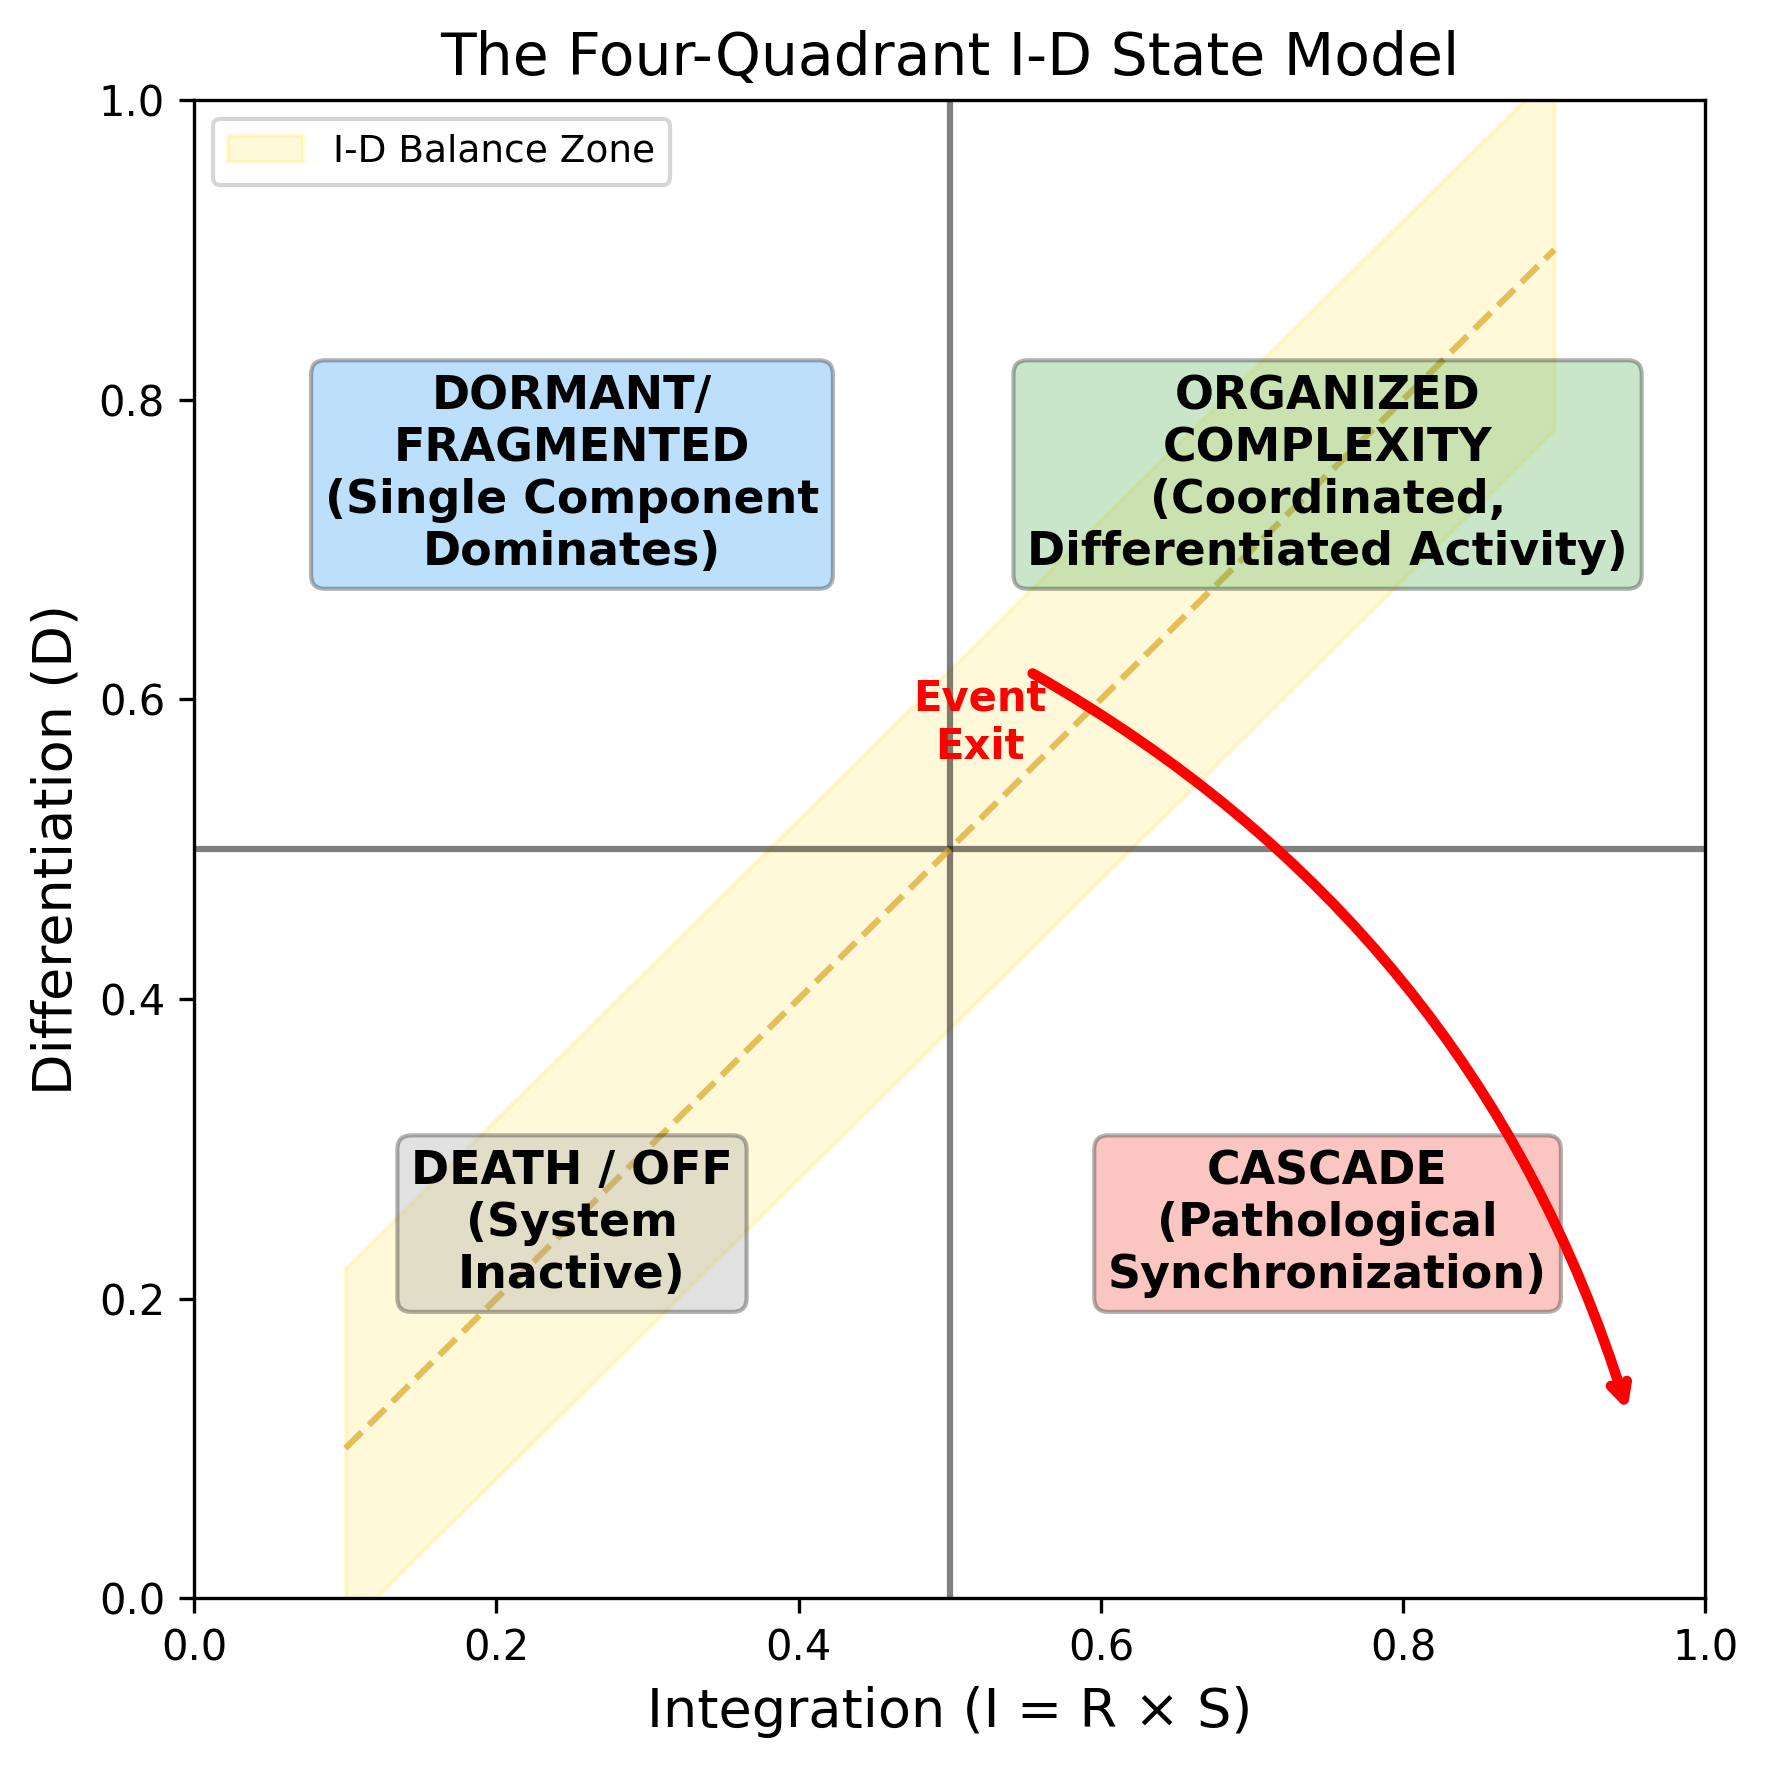
\includegraphics[width=\textwidth]{fig1_quadrant_model.png}
\caption[Schematic of the I-D phase space with four theoretical states and the entropy-coupled axis]{\label{fig:quadrant}Schematic of the $I$--$D$ phase space showing the four theoretical states (Table~I) and the entropy-coupled axis along which empirical observations are constrained. Healthy baseline function occupies the center of this axis; critical events correspond to departures toward the CASCADE or DORMANT extremes.}
\end{figure*}

The Dynamic Existence Threshold (DET) is the boundary of the balance zone in $I$--$D$ space. Systems persist within this zone; critical events correspond to exits from it. We use ``existence'' in the information-theoretic sense: a system \emph{exists as an organized entity} when its integrated information is positive. When $I$--$D$ balance breaks, the system persists physically but its organizational identity---the coordinated structure that distinguishes it from its components---degrades. A market in cascade is still a market in name; it is not functioning as one. A brain in deep sleep still generates electrical activity; it has lost the cross-frequency coordination that characterizes conscious processing. The threshold is not physical death but organizational dissolution---the loss of what we term \emph{multi-scale coordination}, the property of a complex system whose components are simultaneously integrated and differentiated. Crucially, the approach to this boundary should produce early warning signals---rising variance in the balance metric---consistent with the critical slowing down framework~\cite{scheffer2009}.

This paper tests five predictions derived from the DET hypothesis across three domains (financial markets, space weather, and human EEG) using a common five-layer measurement architecture with zero-parameter tuning between domains. The inclusion of EEG data proves decisive: a simple summation metric anti-predicts brain state (performing worse than chance), while the coupling-structure metric achieves high classification accuracy. This dissociation demonstrates that the $I$--$D$ framework captures organizational structure rather than mere signal magnitude---a distinction invisible to simpler approaches.


\section{Methods}

\subsection{Five-Layer Architecture}

To enable cross-domain comparison without parameter tuning, each domain is decomposed into five measurement layers representing distinct scales or modalities of system activity. The five-layer decomposition follows a principle of hierarchical coverage: layers span from the most local or fundamental process ($L_0$) to the most global or emergent indicator ($L_4$). Table~\ref{tab:layers} specifies the mapping.

\begin{table}[!htbp]
\caption[Five-layer architecture mapping for EEG, space weather, and financial domains]{\label{tab:layers}Five-layer architecture across domains. Space weather acronyms: Disturbance Storm Time (Dst), Planetary K-index (Kp), Auroral Electrojet (AE).}
\begin{ruledtabular}
\begin{tabular}{lp{2.0cm}p{2.0cm}p{2.1cm}}
Layer & EEG Sleep & Space Weather & Financial Markets \\
$L_0$ & Delta (0.5--4\,Hz) & F10.7 solar flux & Stock market stress \\
$L_1$ & Theta (4--8\,Hz) & Solar wind pressure & Sector coherence \\
$L_2$ & Alpha (8--13\,Hz) & Dst index & Cross-sector correlation \\
$L_3$ & Beta (13--30\,Hz) & Kp index & VIX implied volatility \\
$L_4$ & Gamma (30--45\,Hz) & AE index & Flight-to-safety flows \\
\end{tabular}
\end{ruledtabular}
\end{table}

The EEG layers correspond to standard clinical frequency bands~\cite{berry2017,oppenheim1997}. Gamma power was computed with awareness of potential electromyographic (EMG) contamination artifacts at frequencies above 30~Hz~\cite{muthukumaraswamy2013}; however, the framework's reliance on relative coupling rather than absolute power mitigates this concern. Space weather layers span the sun--magnetosphere coupling chain from solar surface (F10.7) through interplanetary medium (solar wind dynamic pressure) to magnetospheric response (Dst, Kp, AE), using NASA OMNI2 data~\cite{papitashvili2020}. Financial layers span from individual equity stress through sector-level coherence to market-wide measures of volatility and risk appetite~\cite{forbes2002}. \textbf{$L_4$ (flight-to-safety)} is the mean $z$-score of safe-haven assets (Treasury bonds, gold, US dollar), following the same $z$-score protocol used for all other layers across all domains. An earlier formulation used a conjunction gate conditioning haven activation on concurrent equity stress; ablation testing (Section~\ref{sec:l4ablation}) demonstrated that this additional logic did not improve classification performance (AUC 0.870 without $L_4$ vs.\ 0.868 with the conjunction gate), so the simpler formulation is used here to maintain consistency with the zero-tuning design.

All layer activations are $z$-scored against a 60-day rolling baseline and clipped to non-negative values. This ensures that only elevated activity relative to recent history registers as layer activation. The rolling baseline window is held constant across domains.

\subsection{Metric Definitions}

Four quantities are computed from the five-layer time series at each time step.

\textbf{Effective number of active layers ($N_\text{eff}$).} Following Hill~\cite{hill1973} and Jost~\cite{jost2006}, the effective number of layers is computed as the exponential of Shannon entropy of the normalized layer magnitudes:
\begin{equation}
N_{\text{eff}} = \exp\left( -\sum_{i=0}^{N-1} p_i \ln p_i \right),
\end{equation}
where $p_i = a_i / \sum_j a_j$ is the normalized activation of layer $i$. $N_\text{eff}$ equals 1 when a single layer carries all activation and equals $N$ when all layers are equally active. A minimum activation threshold $\theta = 2.0$ gates the computation: if $N_\text{eff} < \theta$, both $R$ and $S$ are set to zero. This threshold encodes the requirement that at least two layers must be meaningfully active for integration to be possible. The value $\theta = 2.0$ was set a priori and held constant across all domains without tuning.

\textbf{Redundancy ($R$).} $R$ measures the fraction of processing depth engaged:
\begin{equation}
R = \frac{N_{\text{eff}} - 1}{N - 1} \quad \text{when } N_{\text{eff}} \geq \theta,
\end{equation}
where $N = 5$ is the total number of layers. $R$ ranges from 0 (one dominant layer) to 1 (all layers equally active). The physical interpretation varies by domain: in EEG, high $R$ means multiple frequency bands are simultaneously active; in space weather, high $R$ means multiple layers of the sun--magnetosphere chain are elevated; in finance, high $R$ means stress is distributed across multiple market layers.

\textbf{Synergy ($S$).} $S$ captures the coordination and diversity of inter-layer coupling:
\begin{equation}
S = C \times \left(\frac{1}{2} J + \frac{1}{2} P\right) \quad \text{when } N_{\text{eff}} \geq \theta,
\end{equation}
where the three components are:

\begin{itemize}
\item \textbf{Coverage ($C$):} The fraction of available layers effectively engaged: $C = N_{\text{eff}} / N$.

\item \textbf{Evenness ($J$):} Pielou's evenness index~\cite{pielou1966}, measuring how uniformly activation is distributed: $J = H / H_{\max}$, where $H = -\sum p_i \ln p_i$ is Shannon entropy and $H_{\max} = \ln N$. $J = 0$ when one layer dominates; $J = 1$ when all layers are equally active.

\item \textbf{Pattern diversity ($P$):} The temporal diversity of which layer dominates across sub-windows: $P = |\{d_k : k = 1, \ldots, W\}| / W$, where $d_k = \arg\max_i(a_i)$ within the $k$-th sub-window, and $W$ is the number of sub-windows. For EEG, $W = 8$ sub-windows within each 5-second analysis window. For daily-resolution domains, the trailing 8 days are used. $P = 1/W$ when the same layer dominates every sub-window; $P$ approaches 1 as sub-window dominant-layer diversity increases, reaching a maximum of $\min(N, W)/W$ when every sub-window has a different dominant layer (for $N = 5$ and $W = 8$, $P_{\max} = 5/8 = 0.625$).
\end{itemize}

$S$ ranges from 0 to a practical maximum that depends on $N$ and $W$; for the standard configuration ($N = 5$, $W = 8$), $S_{\max} \approx 0.81$ because $P$ is bounded by $\min(N, W)/W = 0.625$. The equal weighting of $J$ and $P$ ($\frac{1}{2}$ each) is a zero-assumption default---optimizing this weighting per domain would undermine the zero-tuning design. High $S$ requires that inter-layer coupling is widespread, balanced, and temporally variable---a stringent condition that is fragile under system perturbation.

\textbf{Integration ($I$).} The integration metric is defined as the product of redundancy and synergy:
\begin{equation}
I = R \times S.
\end{equation}

This product form ensures that $I$ is high only when both conditions are met: multiple components are active ($R$) \emph{and} they are coordinated in a structured way ($S$). A system with high $R$ but low $S$ has many active layers that are uncoupled---busy but disorganized. A system with low $R$ but high $S$ has strong coupling among a few layers---tightly bound but narrow. Only when both are high does the system exhibit the kind of multi-component coordinated integration that the $I$--$D$ framework posits as necessary for organized complexity. Note, however, that empirically healthy systems (e.g., wakefulness) operate at \emph{moderate} $I$, not maximal $I$; the high-$I$, high-$D$ corner is a theoretical limit rather than an observed regime (see Section~4.1).

The physical meaning of $I = R \times S$ per domain:
\begin{itemize}
\item \textbf{EEG:} High $I$ means multiple frequency bands are simultaneously active \emph{and} their activations are balanced and temporally coordinated. In wakefulness, alpha, beta, theta, and gamma all contribute, with structured inter-band coupling. In N3 deep sleep, delta dominates while other bands are suppressed, yielding low $R$ and near-zero $S$ regardless of total spectral power.
\item \textbf{Space weather:} High $I$ means multiple layers of the sun--magnetosphere chain are simultaneously elevated \emph{and} the elevation is coordinated (e.g., a solar flare that drives solar wind pressure, depresses Dst, raises Kp, and activates auroral electrojets in a synchronized cascade).
\item \textbf{Financial markets:} High $I$ means stress is present across multiple market layers \emph{and} the stress is coordinated rather than idiosyncratic---the hallmark of systemic risk as distinguished from sector-specific shocks~\cite{forbes2002}.
\end{itemize}

\textbf{Differentiation ($D$).} $D$ is computed as the Jensen--Shannon distance of the normalized layer activation vector from the uniform distribution~\cite{lin1991,endres2003}:
\begin{equation}
D = \operatorname{JSD}^{1/2}\left(\mathbf{p} \| \mathbf{u}\right),
\end{equation}
where $\mathbf{p}$ is the normalized layer magnitude vector and $\mathbf{u}$ is the uniform distribution over $N$ layers, with JSD computed using base-2 logarithms so that $D \in [0, 1]$. $D$ is high when layers have unequal activations (the system is differentiated) and low when all layers are equally active (the system is uniform). This is complementary to $R$: high $R$ with high $D$ indicates a system where multiple components are active but with structured inequality, while high $R$ with low $D$ would indicate uniform activation---a state rarely observed in natural systems.

\subsection{Balance Zone Definition}

The $I$--$D$ balance zone is defined in $z$-score space. For each domain, $I$ and $D$ time series are standardized to zero mean and unit variance. The balance metric is:
\begin{equation}
B = |z(I) - z(D)|.
\end{equation}

The balance zone is the region where $B < \sigma_{\text{threshold}}$. Results are reported at three primary threshold levels---$\pm 0.5\sigma$, $\pm 1.0\sigma$, and $\pm 1.5\sigma$ (with $\pm 0.75\sigma$ added in robustness checks, Section~\ref{sec:robustness})---to demonstrate that findings are robust to the specific choice of boundary rather than dependent on a single arbitrary threshold.

\subsection{Derived Quantities}

\textbf{Exit velocity.} The rate of change of the balance metric $B$ between consecutive time steps:
\begin{equation}
V_{\text{exit}} = |B_t - B_{t-1}|.
\end{equation}
High exit velocity indicates rapid departure from the balance zone.

\textbf{Variance of $B$ (early warning signal).} A rolling window variance of the balance metric $B = |z(I) - z(D)|$, computed at multiple look-back horizons (5, 10, 15, 20, 25, and 30 days in time-series domains). Rising variance before an event is a signature of critical slowing down~\cite{scheffer2009,dakos2012}: as the system approaches the basin boundary, perturbations take longer to decay, increasing the variance of fluctuations.

\textbf{Residence time.} The number of consecutive time steps a system remains within the balance zone before exiting. Shorter residence times during event periods versus normal periods indicate that events are associated with a reduced ability to maintain $I$--$D$ balance.

\subsection{Data Sources}

\textbf{Financial markets.} 6,785 trading days spanning 27 years. Twenty-six cascade events (comprising 293 systemic days) were identified using standard criteria including days with CBOE Volatility Index (VIX) $> 2\sigma$ above its trailing mean, cross-sector correlation $> 0.8$, and Merrill Lynch Option Volatility Estimate (MOVE) index spikes, corresponding to well-documented market stress episodes (e.g., 2008 financial crisis, 2020 COVID crash, 2010 flash crash). Layer construction used daily data for equity indices, sector exchange-traded funds (ETFs), VIX, and Treasury--equity correlations.

\textbf{Space weather.} 9,802 days of NASA OMNI2 hourly data averaged to daily resolution~\cite{papitashvili2020}. Fifty-one storm days from 26 geomagnetic storm events were identified using the standard Dst $< -50$~nT criterion~\cite{gonzalez1994} (where Dst is the Disturbance Storm Time index, a measure of magnetospheric ring current intensity), consistent with moderate-to-severe storm classification.

\textbf{EEG.} 50 subjects (57,212 total epochs, of which 43,342 Wake and 1,676 N3 were used in the analysis) from the Sleep-EDF dataset on PhysioNet~\cite{kemp2000,goldberger2000}. Wake and N3 deep sleep epochs were extracted using expert-scored hypnograms following American Academy of Sleep Medicine (AASM) criteria~\cite{berry2017}. Each 30-second epoch was decomposed into the five frequency bands of Table~\ref{tab:layers} via bandpass filtering. Band power was computed within six non-overlapping 5-second windows per epoch; the pattern diversity metric $P$ (Section~2.2) was calculated over $W = 8$ windows using the trailing two windows from the preceding epoch to maintain temporal context.

\subsection{Statistical Tests}

All $p$-values are computed using non-parametric methods: Mann--Whitney $U$ tests for group comparisons and permutation tests (10,000 iterations) for variance ratios. AUC values are computed using standard receiver operating characteristic (ROC) analysis. Bootstrap 95\% confidence intervals (1,000 iterations) are reported for key AUC estimates. Benjamini--Hochberg false discovery rate (FDR) correction~\cite{benjamini1995} is applied across all 96 reported $p$-values. All 64 tests significant at $p < 0.05$ remain significant after FDR correction, and no tests lost significance.

\subsection{Zero Parameter Tuning}

A critical design principle of this study is that no parameters are tuned between domains. The five-layer architecture, the metric definitions ($R$, $S$, $D$, $I$), the balance zone thresholds, and the statistical tests are identical across financial, space weather, and EEG domains. The only domain-specific element is the mapping from raw data to the five layers (Table~\ref{tab:layers}), which is determined by the physics of each domain rather than by optimization. This constraint is deliberately restrictive: a framework that requires per-domain calibration would be of limited theoretical interest, as it would leave open the possibility that apparent cross-domain consistency is an artifact of fitting.


\section{Results}

\subsection{Test 1: $I$--$D$ Phase Space Structure}

The first prediction of the DET framework is that the $I$--$D$ phase space should exhibit characteristic structure: events should cluster at the extremes (high $I$ / low $D$ or low $I$ / high $D$), while normal states should occupy the center.

Across all three domains, $I$ and $D$ show a clean negative correlation within event periods: as $I$ rises, $D$ falls. This anticorrelation is principally a mathematical consequence of the chosen proxies: $R$ (a component of $I$) increases with the Shannon entropy $H$ of the layer distribution, while $D$ (JSD from uniform) decreases with $H$. The metrics are thus entropy-coupled rather than fully independent (Section~3.6.4). The strength of this coupling varies across system states, with implications discussed in Section~3.6.4.

To quantify the directional dynamics, each time step was classified into one of four categories based on the signs of $dI$ and $dD$ (the one-step changes in $I$ and $D$):

\begin{itemize}
\item \textbf{CASCADE} ($dI > 0$, $dD < 0$): Integration rising while differentiation falls---the signature of pathological synchronization.
\item \textbf{RECOVERY} ($dI < 0$, $dD > 0$): Integration falling while differentiation rises---return toward normal.
\item \textbf{COINCIDENCE} ($dI > 0$, $dD > 0$): Both rising simultaneously.
\item \textbf{COLLAPSE} ($dI < 0$, $dD < 0$): Both falling simultaneously.
\end{itemize}

The CASCADE category is strongly enriched during events: 45--51\% of event time steps fall in this category, compared to 21--34\% of normal time steps. The COINCIDENCE category---in which both $I$ and $D$ rise simultaneously---accounts for less than 2\% of event time steps, indicating that the budget constraint between $I$ and $D$ is nearly absolute during critical periods.

Perhaps most striking, events systematically flee the balance zone. In space weather, only 17.6\% of event time steps occupy the balance zone (at $\pm 1.0\sigma$), compared to 44.9\% of normal time steps---a 2.5$\times$ depletion during events. This depletion is consistent across all three domains, confirming the DET prediction that critical events correspond to departures from $I$--$D$ balance.

\subsection{Test 2: Residence Time Discrimination}

The second prediction is that events should exit the balance zone faster than normal state changes---that is, residence times within the balance zone should be shorter during event periods.

\textbf{Financial markets.} At the $\pm 1.5\sigma$ balance zone boundary, the median residence time during normal periods is 2 days, while during event periods it is 1 day (Mann--Whitney $U$ test, $p = 0.0001$). This indicates that event periods are characterized by a halving of the system's ability to maintain $I$--$D$ balance.

\textbf{Space weather.} At the $\pm 1.5\sigma$ boundary with Sum as the $I$ coordinate, the median residence time during normal periods is 3 days, compared to 2 days during event periods ($p = 0.01$). Using a kernel density estimation (KDE)-based adaptive boundary, the financial result remains significant ($p = 0.0003$), but the space weather result does not reach significance ($p = 0.66$), suggesting that the fixed-threshold approach is more robust for this domain.

The residence time results are reported at multiple thresholds in Table~\ref{tab:residence}; distributions are shown in Fig.~\ref{fig:residence}.

\begin{table}[!htbp]
\caption[Balance zone residence time in median days by domain and threshold]{\label{tab:residence}Balance zone residence time (median days) by domain and threshold.}
\begin{ruledtabular}
\begin{tabular}{lllll}
Domain & Threshold & Normal & Event & $p$-value \\
Financial & $\pm 1.5\sigma$ & 2 & 1 & 0.0001 \\
Financial & KDE & 2 & 1 & 0.0003 \\
Space & $\pm 1.5\sigma$ & 3 & 2 & 0.01 \\
\end{tabular}
\end{ruledtabular}
\end{table}

\begin{figure*}[t]
\centering
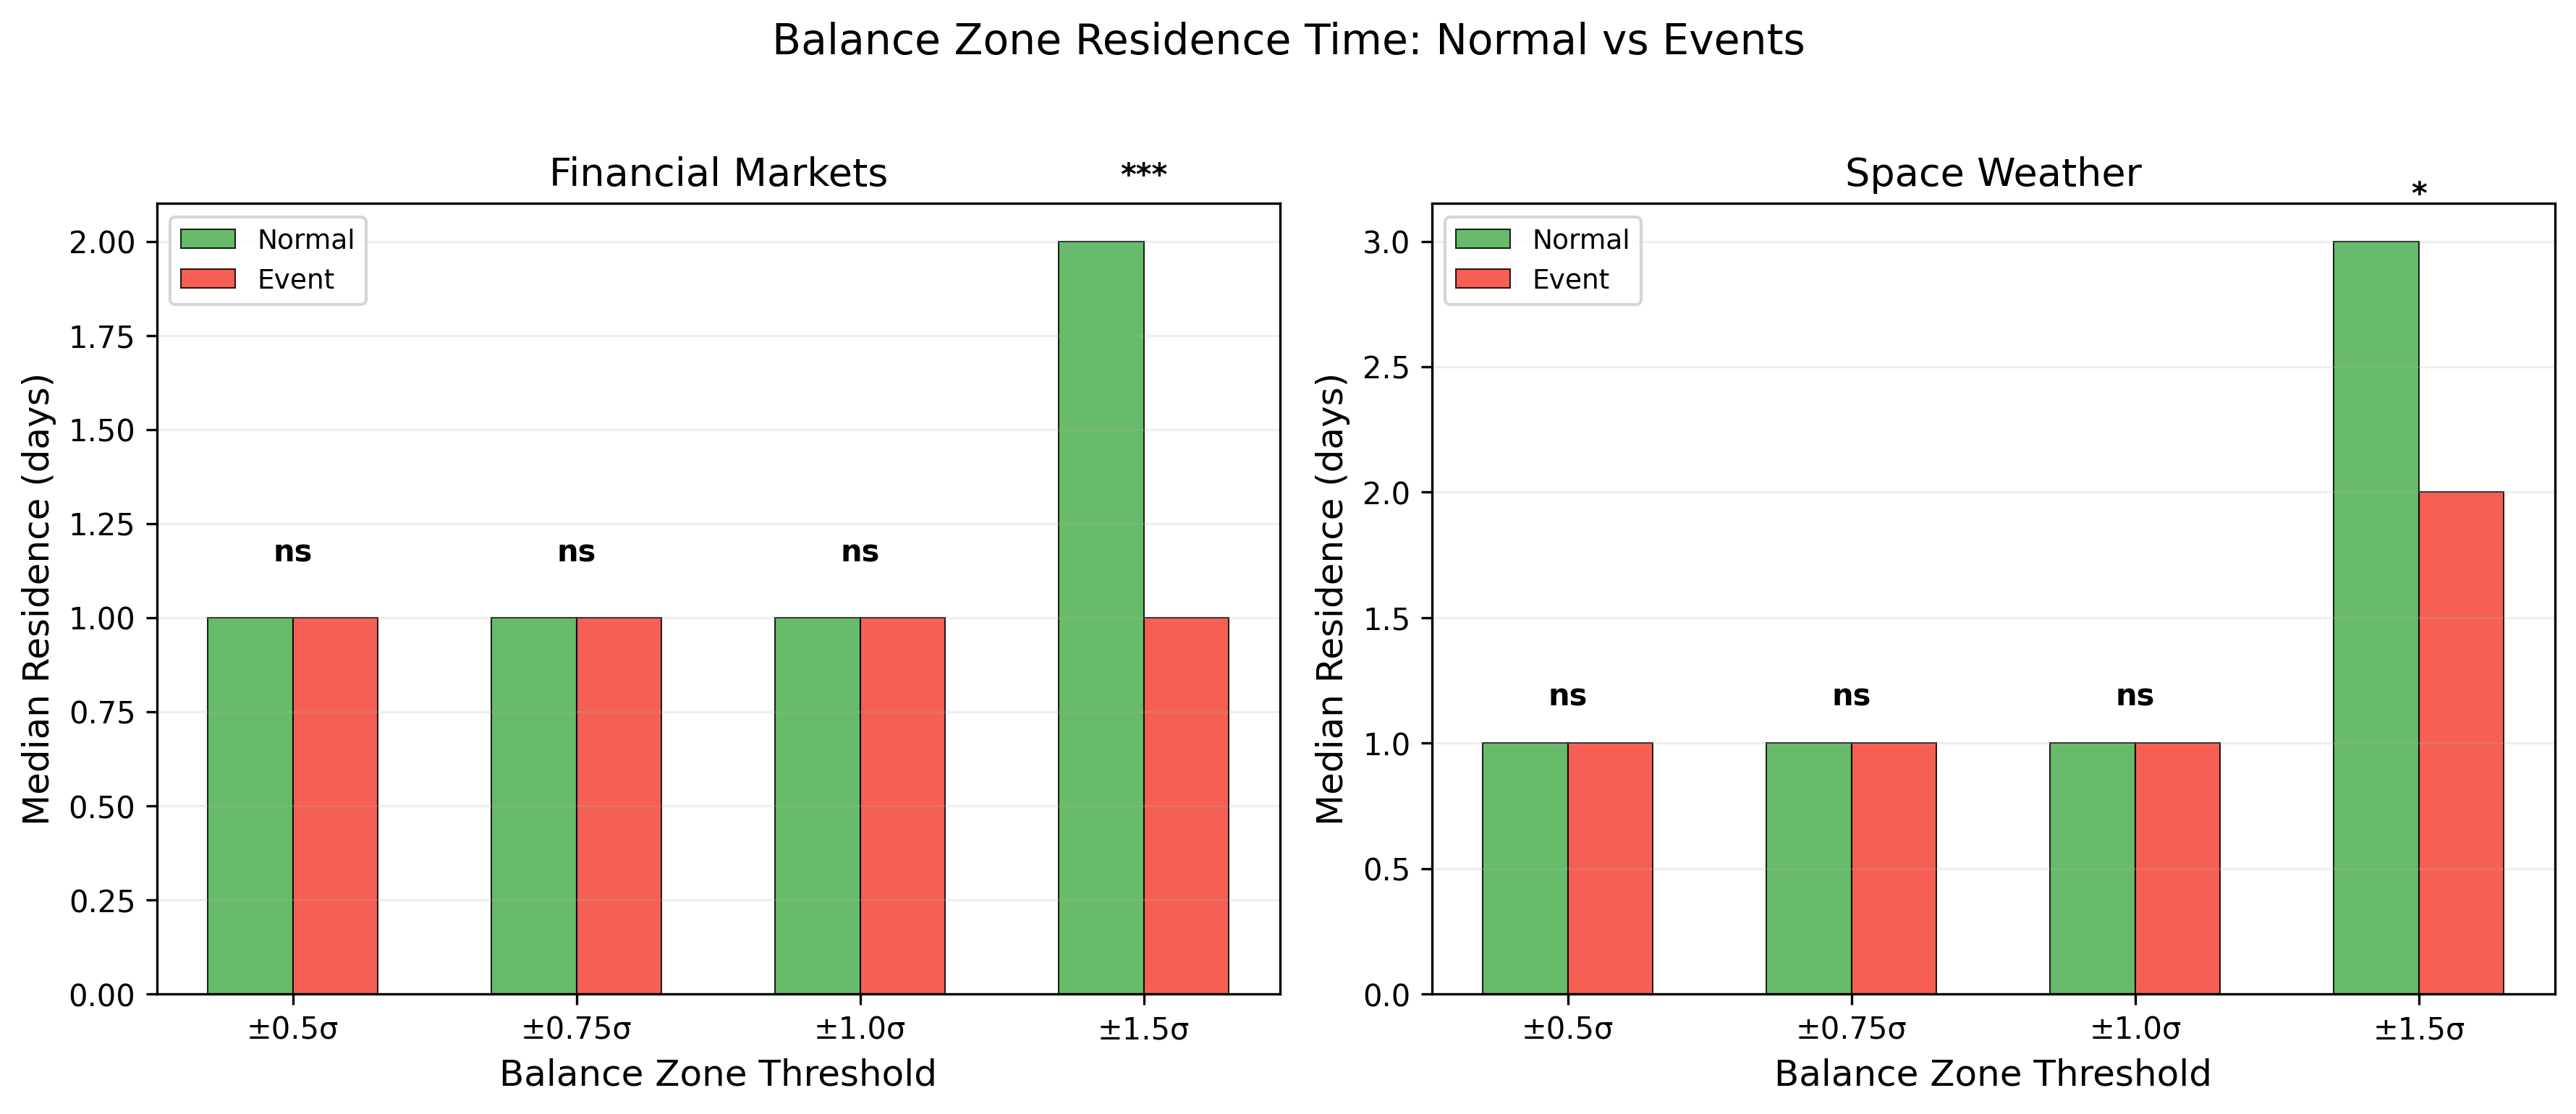
\includegraphics[width=\textwidth]{fig5_residence.png}
\caption[Balance zone residence time distributions comparing event and normal periods]{\label{fig:residence}Balance zone residence time distributions for event vs.\ normal periods. Events exit the balance zone faster than normal state changes, with median residence times halved during event periods in financial markets ($p = 0.0001$).}
\end{figure*}

The discrimination improves at wider thresholds, consistent with the interpretation that larger balance zones capture more of the normal-state dynamics while still showing rapid event-period exits.

\subsection{Test 3: Early Warning Signal}

The third and most practically significant prediction is that rising variance of the balance metric $B$ should precede events, providing an early warning signal. This prediction connects the DET framework directly to the critical transitions literature: as a system approaches the boundary of its balance zone, its fluctuations should grow---the hallmark of critical slowing down~\cite{scheffer2009,dakos2012}.

\textbf{Financial markets.} The 30-day rolling variance of $B$ shows a 2.0$\times$ elevation at a 5-day lead before cascade events relative to matched normal periods (permutation test, $p < 0.0001$). The elevation persists at 10-day (1.9$\times$, $p < 0.001$), 15-day (1.8$\times$, $p < 0.001$), and 30-day (1.4$\times$, $p < 0.01$) leads. The gradual decay of the signal over longer horizons is expected: the early warning should be strongest close to the event and weaken with distance.

\textbf{Space weather.} The same metric shows a 2.0$\times$ elevation at a 5-day lead ($p = 0.0002$), consistent with financial markets in both magnitude and significance. However, the signal fades more rapidly, losing significance by the 15-day horizon. This faster decay is physically sensible: geomagnetic storms develop over days rather than the weeks-to-months timescale of financial cascades.

The convergence of the 2.0$\times$ elevation ratio across two physically unrelated domains at the 5-day horizon---without any parameter tuning---is notable (Fig.~\ref{fig:early_warning}). The $I$--$D$ balance metric appears to provide a common coordinate system in which the approach to critical transitions manifests with quantitatively similar early warning signatures.

\begin{figure*}[t]
\centering
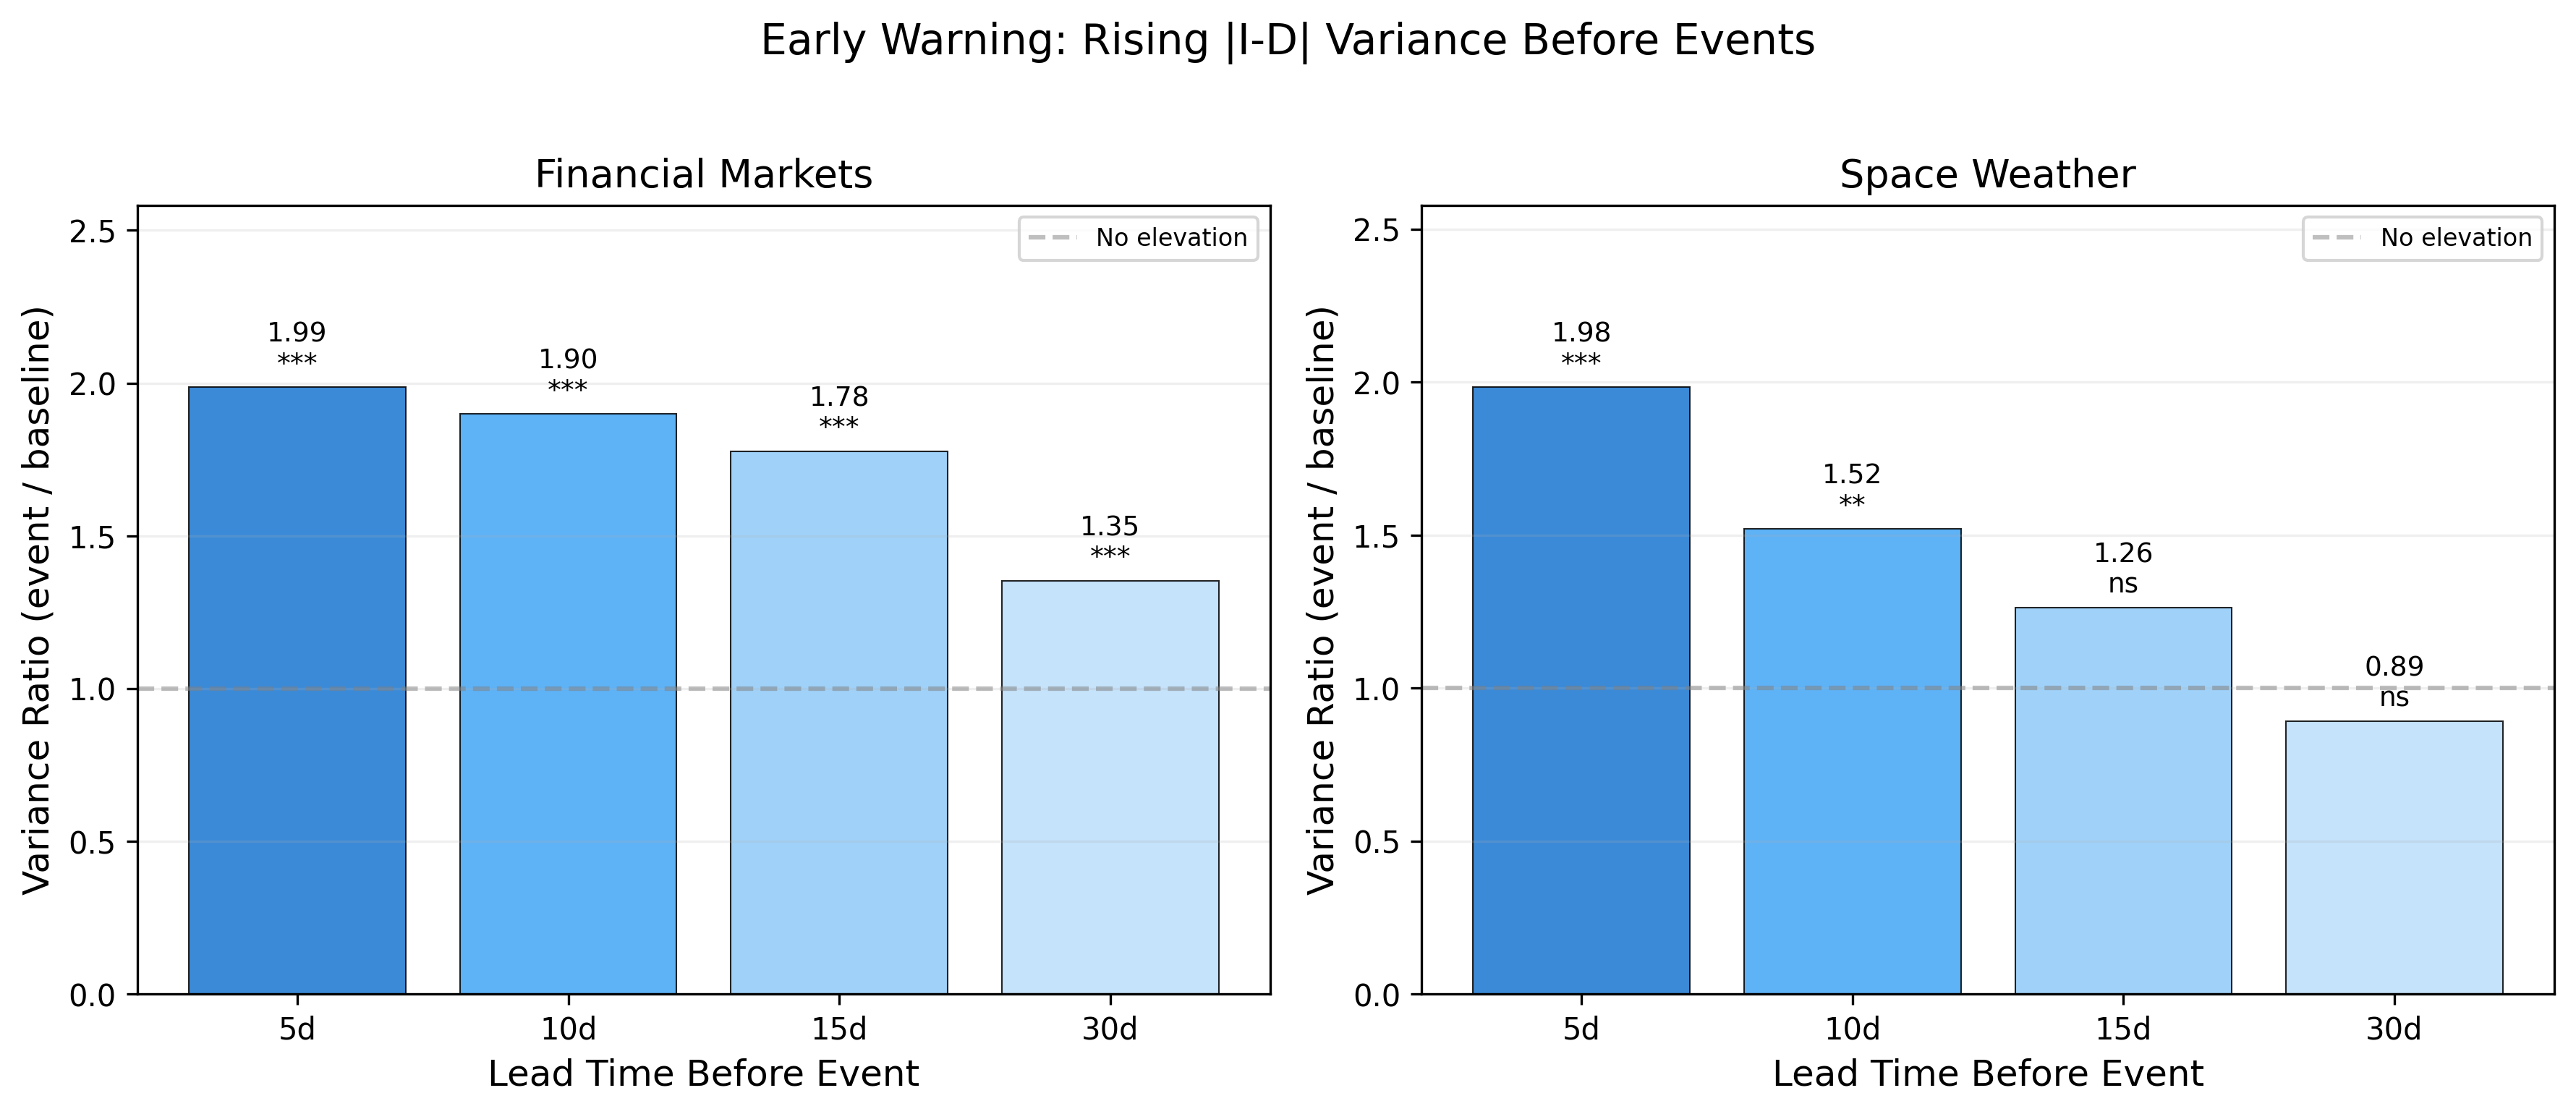
\includegraphics[width=\textwidth]{fig2_early_warning.png}
\caption[Rolling variance of the balance metric showing pre-event elevation in financial and space weather domains]{\label{fig:early_warning}Rolling variance of the balance metric $B = |z(I) - z(D)|$ showing pre-event elevation. The 30-day rolling variance rises to 2.0$\times$ its normal-period level at a 5-day lead before events in both financial and space weather domains, consistent with critical slowing down.}
\end{figure*}

\subsection{Test 4: Classifier Performance, Exit Velocity, and Cross-Domain Transfer}

\textbf{Exit velocity as a discriminator.} Exit velocity---the rate of change of the balance metric---discriminates events from normal periods with AUC 0.692 in financial markets and AUC 0.843 in space weather ($p < 1 \times 10^{-17}$ for both). The higher AUC in space weather likely reflects the sharper onset dynamics of geomagnetic storms compared to the more diffuse build-up of financial cascades.

\textbf{Sum as a baseline.} The simple sum of all five layers ($\text{Sum} = L_0 + L_1 + L_2 + L_3 + L_4$) provides a strong baseline classifier: AUC 0.868 for financial cascades and AUC 0.932 for space weather storms. This is expected---during cascades, most or all layers are elevated, so their sum naturally discriminates. The relevance of this baseline will become clear in the EEG analysis (Section~\ref{sec:eeg}), where Sum fails catastrophically.

\textbf{Composite classifier.} Combining exit velocity with the 30-day variance signal yields a composite classifier with AUC 0.798 (financial) and 0.886 (space weather). The composite does not exceed Sum alone in these domains because the dominant signal during financial and space weather cascades is total magnitude---a signal that Sum captures directly.

A comparison of classifier performance across metrics and domains is shown in Fig.~\ref{fig:classifier}.

\begin{figure*}[t]
\centering
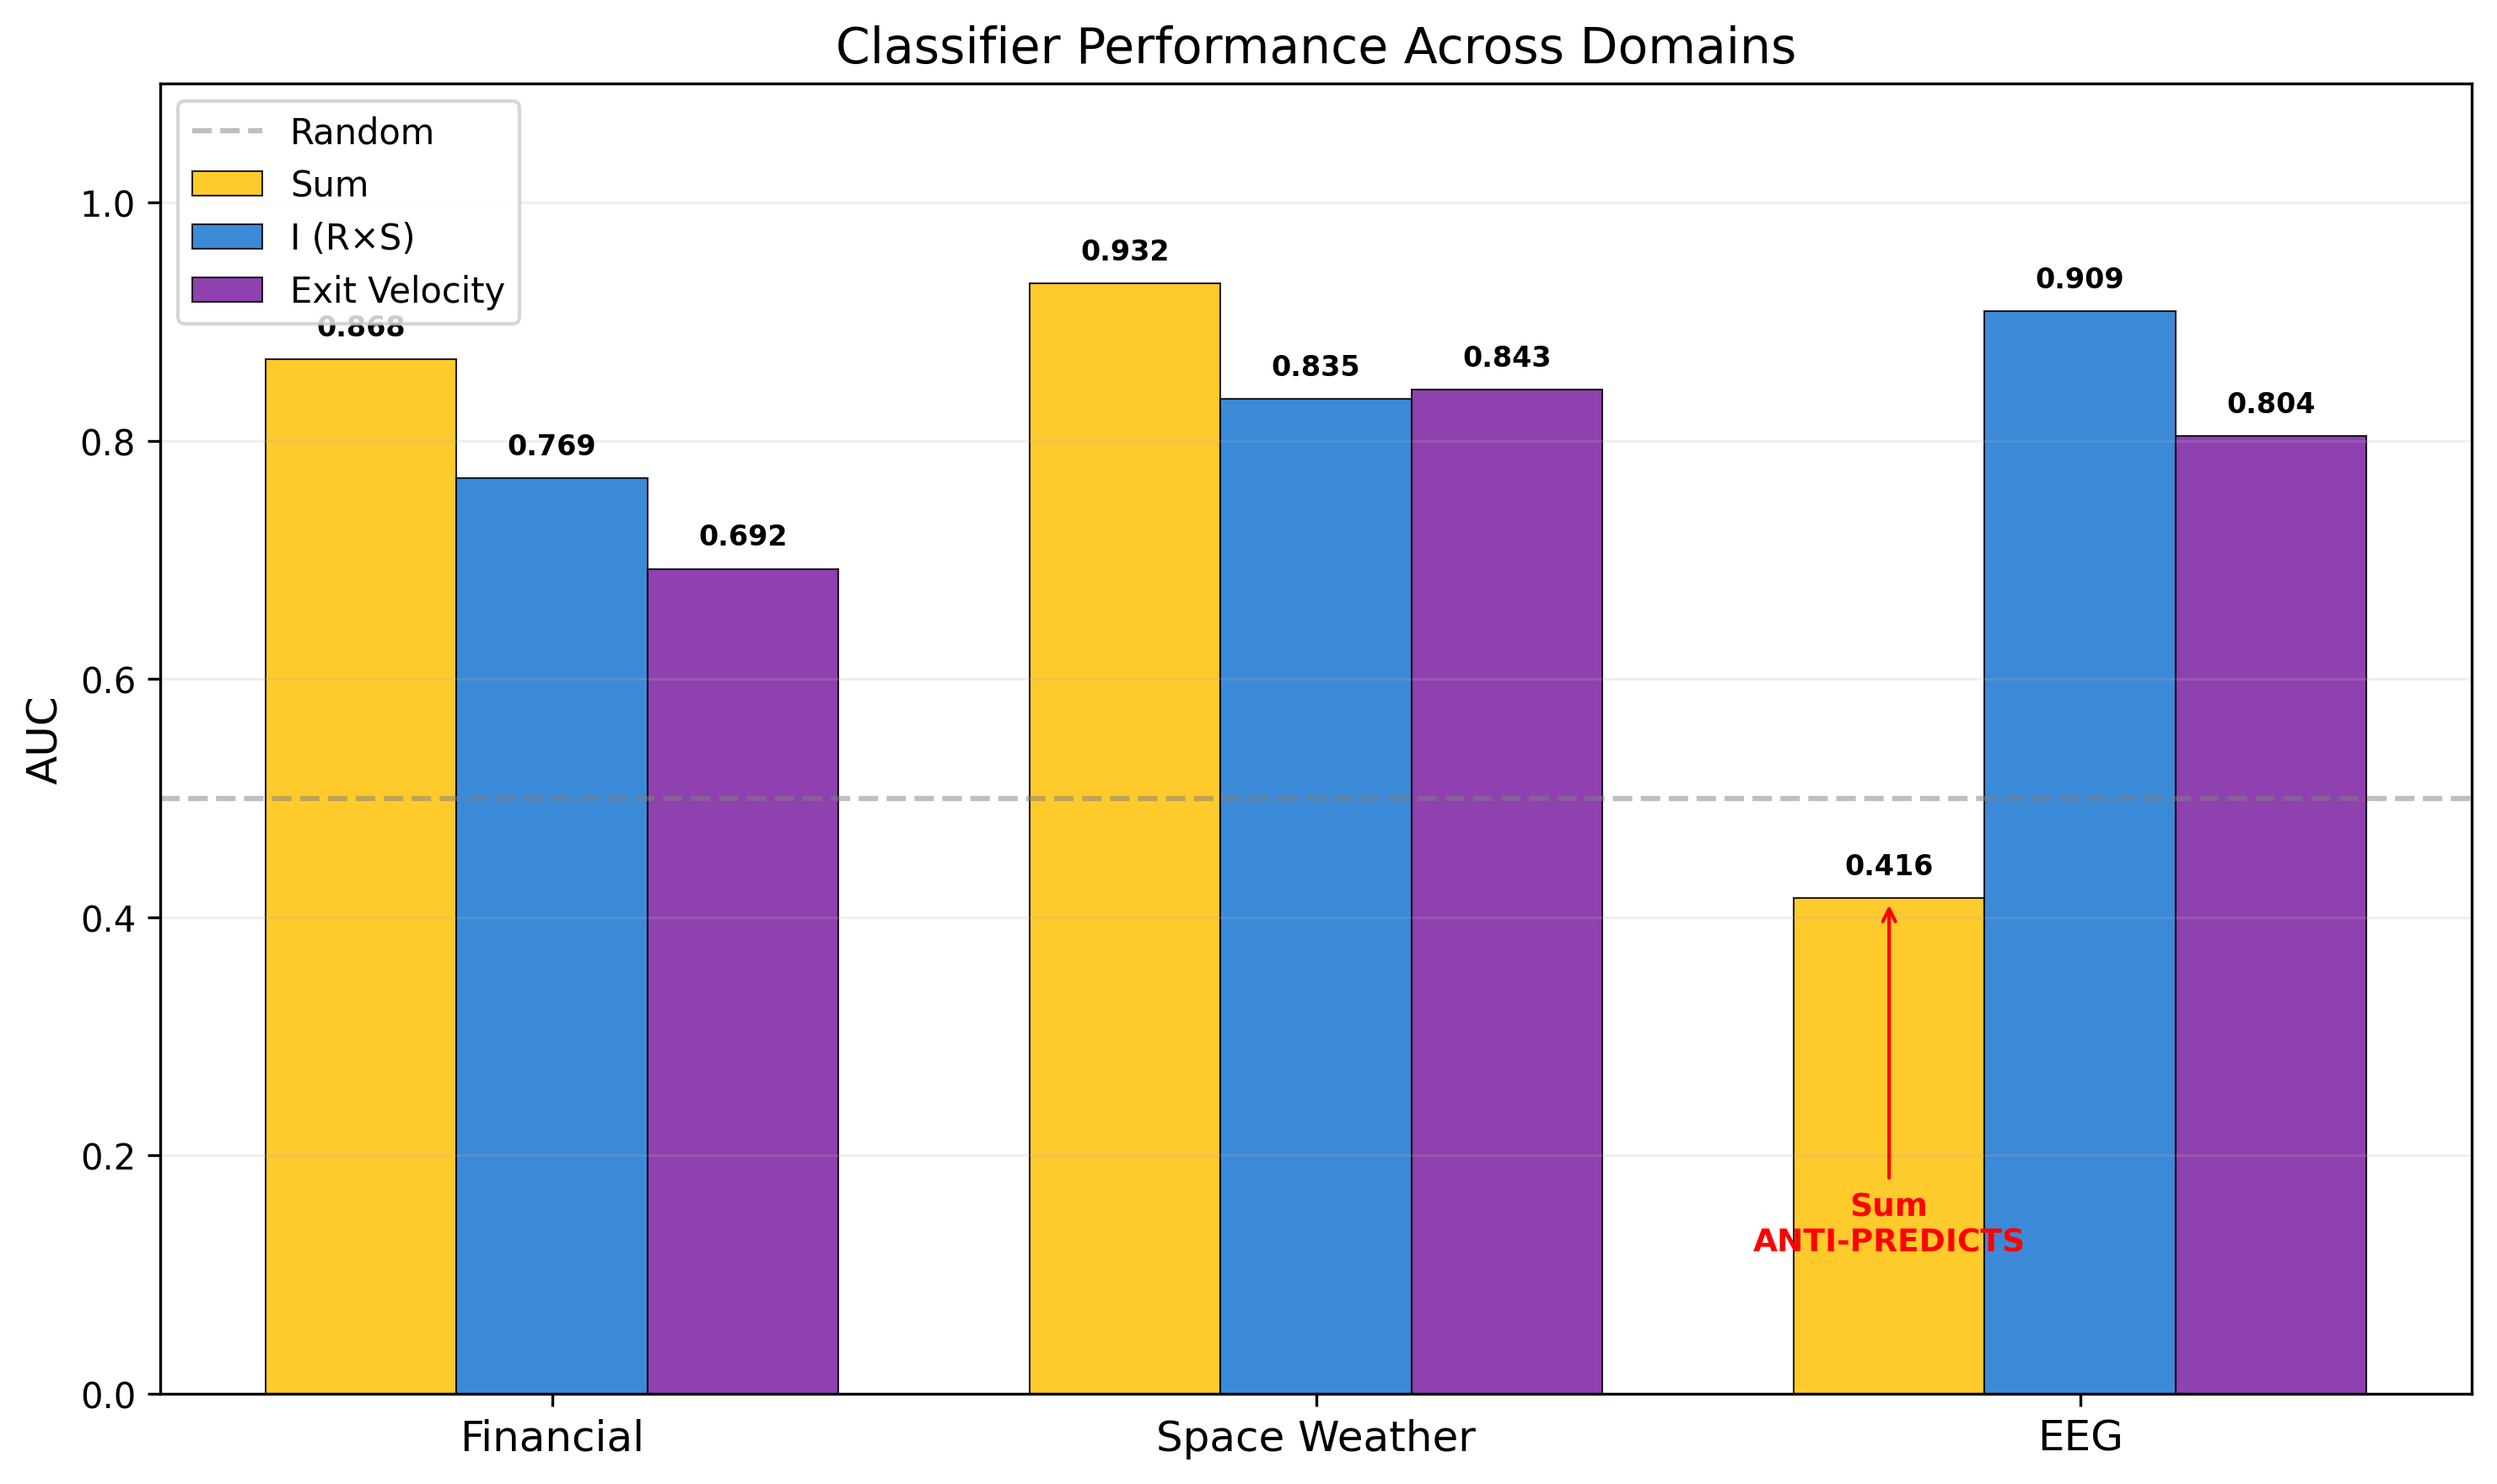
\includegraphics[width=\textwidth]{fig3_classifier_comparison.png}
\caption[Classifier comparison across metrics and domains showing Sum, R times S, and exit velocity performance]{\label{fig:classifier}Classifier comparison across metrics (Sum, $R \times S$, exit velocity) and domains (financial markets, space weather). Sum provides a strong baseline in time-series domains but anti-predicts in EEG, while exit velocity and $R \times S$ capture structural organization.}
\end{figure*}

\textbf{Cross-domain transfer.} To test whether the framework captures domain-general structure, classification thresholds learned in one domain were applied to the other without recalibration. The Sum-based threshold ratio between domains is 1.47$\times$, and financial-to-space transfer achieves a true positive rate (TPR) of 0.78---reasonable cross-domain performance for a zero-tuning framework. The $R \times S$ threshold ratio is larger (3.77$\times$), reflecting the greater domain-specificity of coupling structure compared to total magnitude. For cross-domain transfer, Sum provides a more stable $I$ coordinate than $R \times S$.

\subsection{\label{sec:eeg}Test 5: EEG---The Crucial Experiment}

The EEG domain provides the most stringent test of the DET framework because, unlike financial markets and space weather, the two states being compared (Wake and N3 deep sleep) differ in their organizational \emph{structure} without necessarily differing in total signal \emph{magnitude}. Indeed, N3 deep sleep is characterized by high-amplitude slow-wave oscillations that produce \emph{higher} total spectral power than wakefulness~\cite{massimini2005}. Any framework that conflates magnitude with organization will fail in this domain. The inclusion of EEG was specifically motivated by this expectation: it is a domain where Sum \emph{should} fail and where $I$--$D$ balance \emph{should} succeed, if the framework is capturing what it claims to capture.

\subsubsection{Five-Subject Pilot}

The pilot analysis of 5 subjects from the Sleep-EDF dataset yielded the following results:

\textbf{Balance zone occupancy.} At the $\pm 0.5\sigma$ threshold, Wake epochs occupy the balance zone 21.4\% of the time, compared to 1.1\% for N3 epochs---an 18.9$\times$ ratio. At the $\pm 1.5\sigma$ threshold, the ratio is 4.5$\times$ (Wake 60.7\% vs.\ N3 13.4\%). The N3 state is almost entirely excluded from the tight balance zone, consistent with the DET prediction that deep sleep corresponds to the low-$I$/high-$D$ (fragmented) quadrant.

\textbf{Mean integration and differentiation.} Mean $I$ ($R \times S$): Wake 0.056, N3 0.002---a 28$\times$ ratio. Mean $D$: Wake 0.556, N3 0.680. Wake has moderate $I$ and moderate $D$, occupying the moderate-entropy region where both metrics take intermediate values consistent with organized multi-band coupling. N3 has near-zero $I$ and elevated $D$, occupying the dormant/fragmented region where a single layer (delta) dominates. The 28$\times$ ratio in $I$ reflects the near-total collapse of cross-band coupling in N3: delta dominates while theta, alpha, beta, and gamma are suppressed, yielding minimal redundancy and near-zero synergy.

\textbf{Exit velocity.} Wake epochs show mean exit velocity of 0.558 compared to 0.133 for N3 (4.2$\times$ ratio, $p = 1.7 \times 10^{-114}$). The large effect size reflects the dynamic richness of wakefulness---the $I$--$D$ balance point shifts continuously as attentional and cognitive states fluctuate---compared to the static, delta-dominated landscape of N3.

\textbf{The Sum anti-prediction.} This is the headline finding. The simple sum of spectral power across all five frequency bands yields an AUC of 0.288 for discriminating Wake from N3. An AUC below 0.5 means the classifier is \emph{anti-predicting}: it systematically assigns higher scores to N3 than to Wake because N3 has higher total spectral power. Sum is not merely uninformative---it is actively misleading. By contrast, $I$ ($R \times S$) achieves AUC 0.869, and exit velocity achieves AUC 0.793.

This result is not a statistical fluke. It follows directly from the physiology of sleep. N3 deep sleep is dominated by high-amplitude delta oscillations (0.5--4~Hz), which are generated by thalamocortical circuits during the slow oscillation~\cite{massimini2005}. These waves have amplitudes 2--5$\times$ larger than typical waking EEG~\cite{niedermeyer2005}, producing high total power. But this power is concentrated in a single frequency band: delta accounts for $>$80\% of total spectral power in N3. $R$ is therefore near its minimum (one active layer), and $S$ is near zero (synergy requires multiple coupled components). The product $R \times S$ correctly identifies N3 as a state of low integration---many neurons firing in synchrony at one frequency, with no cross-band coordination.

Wakefulness, by contrast, has moderate power distributed across multiple bands: alpha contributes during relaxed attention, beta during active processing, theta during memory encoding, and gamma during binding operations~\cite{buzsaki2006}. $R$ is moderate (several active layers), and $S$ is moderate (structured inter-band coupling). The product $R \times S$ correctly identifies wakefulness as a state of moderate integration---the moderate-entropy baseline of the $I$--$D$ framework, where both metrics take intermediate values and multiple components are simultaneously active and coupled. This is not the high-$I$, high-$D$ ``organized complexity'' corner of the theoretical four-state model (which is inaccessible under entropy coupling; Section~4.1), but rather the empirically healthy region at the center of the entropy axis.

Sum conflates magnitude with structure. $R \times S$ captures the coupling structure that the $I$--$D$ framework posits as fundamental. The EEG domain provides a clean dissociation between the two, confirming that the framework is measuring what it claims to measure.

\subsubsection{Fifty-Subject Scale-Up}

The analysis was scaled to 50 subjects (57,212 epochs) to assess stability. Key results:

\textbf{Balance zone occupancy.} At the $\pm 0.5\sigma$ threshold, Wake occupies the balance zone 17.5\% of the time, compared to 0.5\% for N3---a 36.6$\times$ ratio. The larger ratio at 50 subjects (vs.\ 18.9$\times$ at 5 subjects) reflects both the increased Wake sample providing a more stable occupancy estimate and the greater N3 exclusion from the tight balance zone in the larger, more representative cohort. At $\pm 1.5\sigma$, Wake is 53.9\% vs.\ N3 4.3\% (12.5$\times$).

\textbf{$I$ ($R \times S$) AUC.} 0.909, with bootstrap 95\% confidence interval [0.904, 0.913]. The improvement from 0.869 (5 subjects) to 0.909 (50 subjects) indicates that the signal strengthens with additional data, consistent with a genuine population-level effect rather than subject-specific artifacts.

\textbf{Sum AUC.} 0.416---still anti-predicting (below 0.5), consistent across sample sizes (0.288 at 5 subjects, 0.416 at 50 subjects).

\textbf{Exit velocity ratio.} 4.9$\times$ (up from 4.2$\times$ at 5 subjects), confirming the signal across a larger population.

\begin{table}[!htbp]
\caption[EEG results summary across 5, 30, and 50 subject sample sizes]{\label{tab:eeg}EEG results summary across sample sizes. \textbf{Boldface} denotes final results from the full 50-subject cohort. The 50-subject $I$ AUC has 95\% CI [0.904, 0.913]; Sum AUC below 0.5 indicates anti-prediction. Balance ratio at 30 subjects is undefined (N3 occupancy = 0\%).}
\begin{ruledtabular}
\begin{tabular}{p{2.4cm}lll}
Metric & 5 Subj. & 30 Subj. & 50 Subj. \\
$I$ ($R{\times}S$) AUC & 0.869 & 0.904 & \textbf{0.909} \\
Sum AUC & 0.288 & 0.330 & \textbf{0.416} \\
Balance ratio ($\pm 0.5\sigma$) & 18.9$\times$ & --- & \textbf{36.6$\times$} \\
Exit vel.\ ratio & 4.2$\times$ & 5.6$\times$ & \textbf{4.9$\times$} \\
\end{tabular}
\end{ruledtabular}
\end{table}

The distribution of $I$ ($R \times S$) for Wake vs.\ N3 is shown in Fig.~\ref{fig:eeg_stages}, illustrating the anti-prediction of Sum and the clean separation achieved by the coupling metric.

\begin{figure*}[t]
\centering
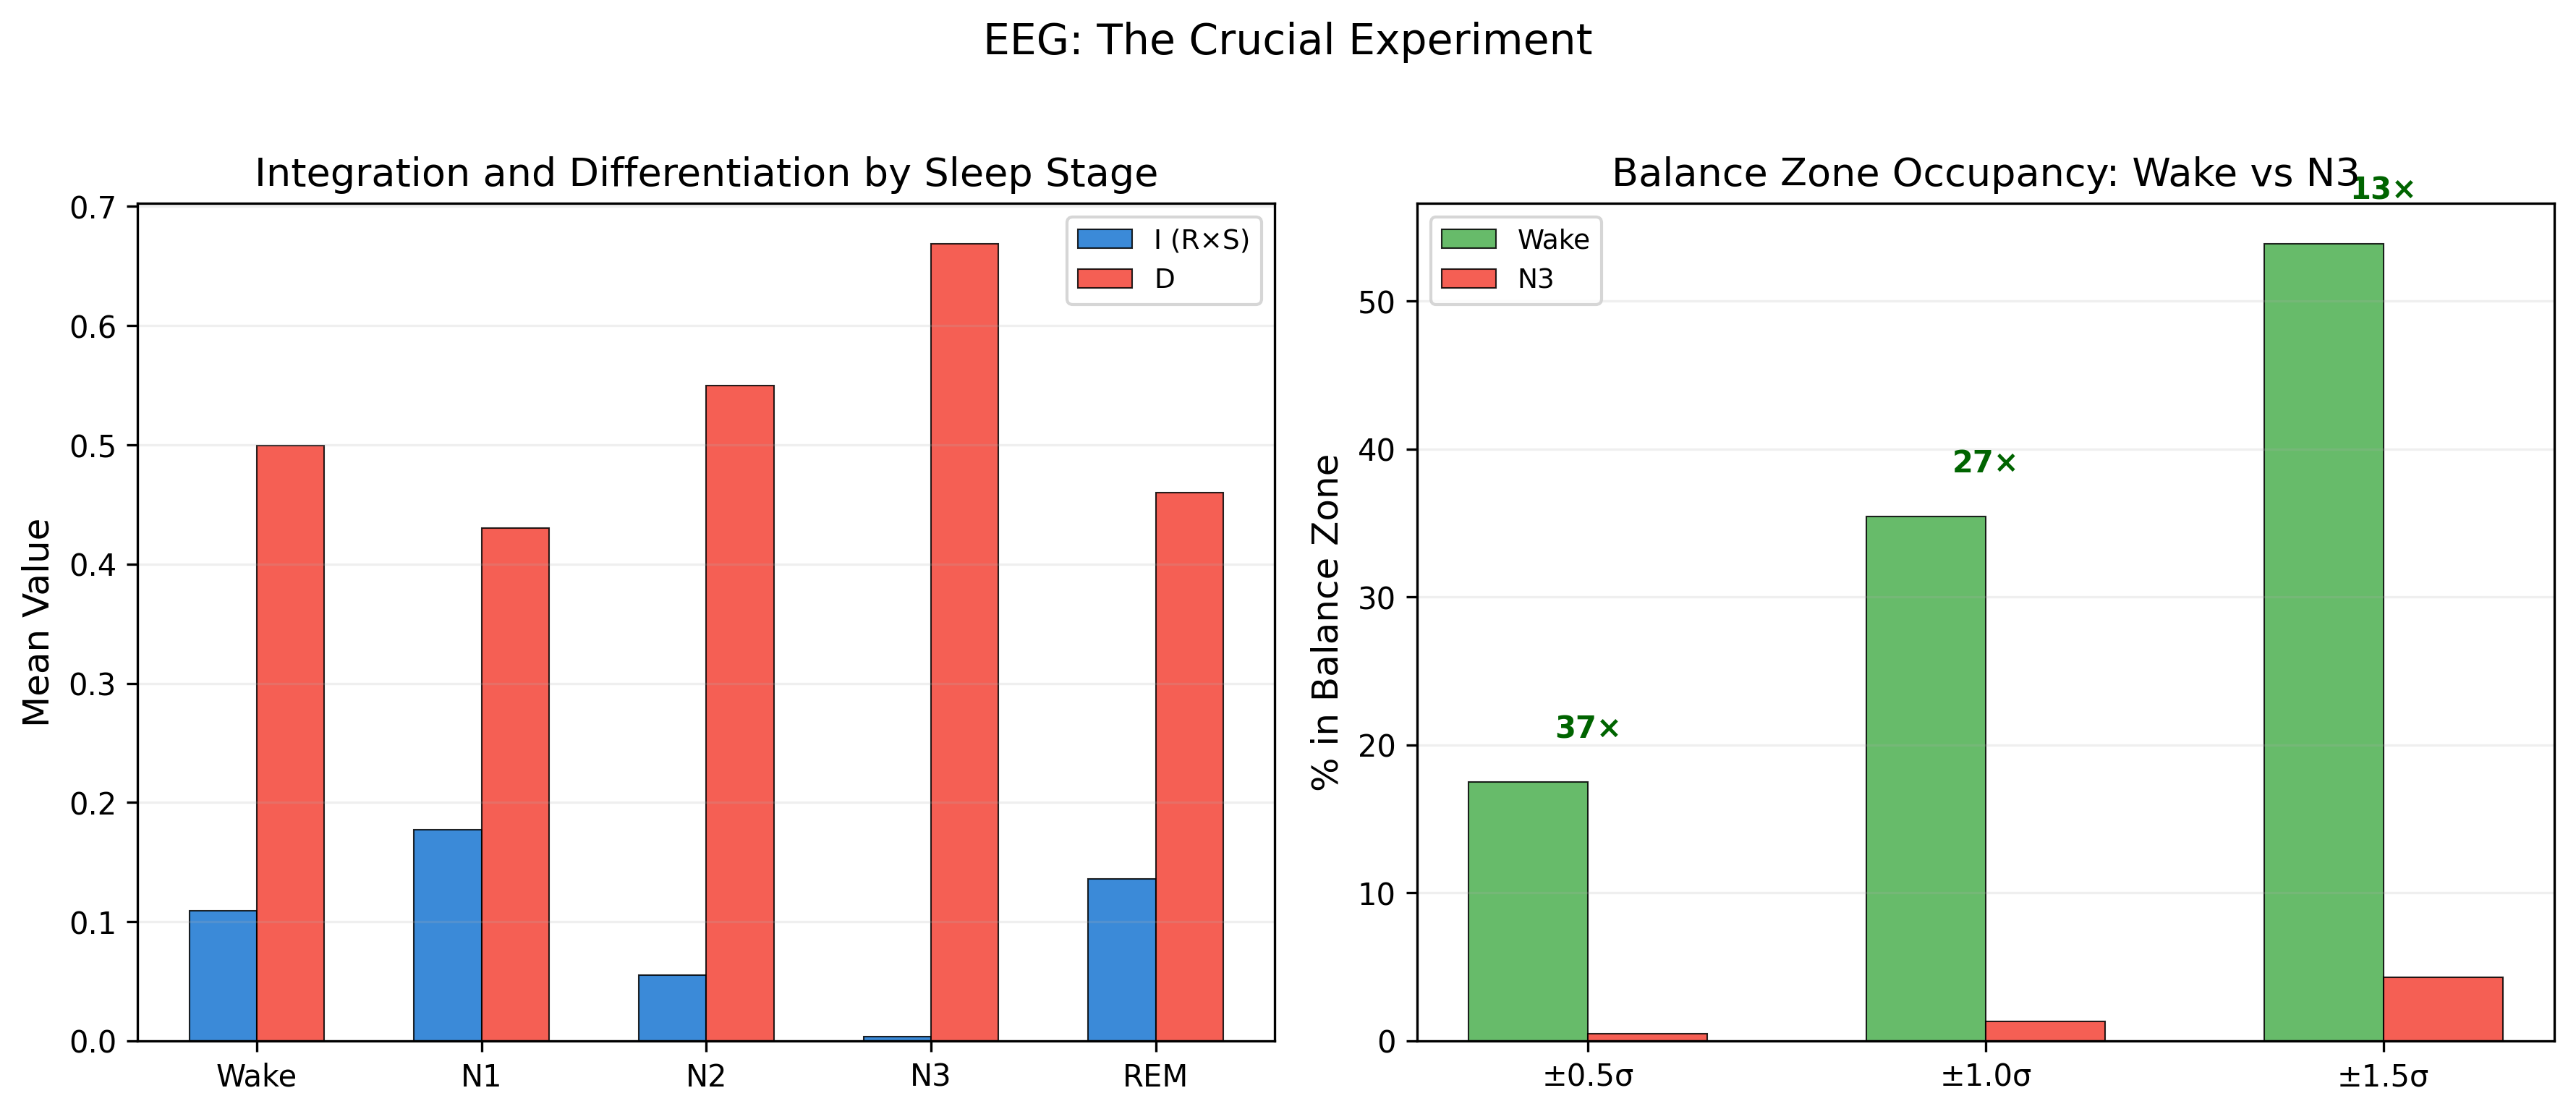
\includegraphics[width=\textwidth]{fig4_eeg_stages.png}
\caption[Distribution of I for Wake versus N3 deep sleep showing clean separation by the coupling metric]{\label{fig:eeg_stages}Distribution of $I$ ($R \times S$) for Wake vs.\ N3 deep sleep across 50 subjects (57,212 epochs). The coupling metric cleanly separates states (AUC 0.909), while Sum anti-predicts (AUC 0.416) because N3 has higher total spectral power than wakefulness.}
\end{figure*}

\subsection{\label{sec:robustness}Robustness Across Thresholds}

A legitimate concern with any threshold-based analysis is sensitivity to the specific threshold chosen. To address this, all key results were computed at four balance zone thresholds: $\pm 0.5\sigma$, $\pm 0.75\sigma$, $\pm 1.0\sigma$, and $\pm 1.5\sigma$.

\textbf{Balance zone occupancy discrimination} (events vs.\ normal, or Wake vs.\ N3) is significant at all four thresholds in all three domains. The discrimination is strongest at tight thresholds ($\pm 0.5\sigma$) and weakens gradually at wider thresholds, as expected---a wider balance zone admits more of both event and normal states.

\textbf{Residence time discrimination} is significant at $\pm 1.5\sigma$ in financial markets ($p = 0.0001$) and in space weather ($p = 0.01$). At narrower thresholds ($\pm 1.0\sigma$ and below), median residence times in both conditions are 1 day, yielding insufficient resolution for discrimination. The KDE-based adaptive boundary confirms the financial result ($p = 0.0003$) but not the space weather result ($p = 0.66$), suggesting that fixed wide thresholds are more robust for the space domain.

\textbf{Sum anti-prediction in EEG} is present at all thresholds tested. The AUC of Sum for Wake vs.\ N3 classification remains below 0.5 (ranging from 0.288 at 5 subjects to 0.416 at 50 subjects) regardless of balance zone definition, because the anti-prediction is driven by spectral power distribution rather than balance zone thresholds.

\textbf{Early warning signal} elevation is significant at all thresholds in financial markets and at $\pm 1.0\sigma$ and $\pm 1.5\sigma$ in space weather. The 2.0$\times$ elevation ratio at 5-day lead is stable to within $\pm 0.2\times$ across threshold choices.

These results confirm that the DET framework's findings are not artifacts of a particular threshold choice. The qualitative conclusions---events flee balance, residence time shortens during events, Sum anti-predicts in EEG, early warning variance rises before events---hold across a threefold range of threshold values.

\subsubsection{Negative Controls}

To confirm that the observed discriminative power reflects genuine structure rather than statistical artifacts, two permutation controls were conducted.

\textbf{Label shuffle.} Event labels were randomly permuted 1,000 times while layer values were held fixed. For financial data, the real AUC (Sum) of 0.868 dropped to a shuffle mean of $0.500 \pm 0.017$ (permutation $p < 0.001$). For space weather, the real AUC of 0.932 dropped to $0.501 \pm 0.041$ ($p < 0.001$). Exit velocity showed identical null behavior (shuffle AUC 0.500 in both domains). These results confirm that the classifiers are detecting genuine label-correlated structure, not distributional artifacts.

\textbf{Temporal layer shuffle.} The temporal ordering of each layer was independently permuted (200 iterations), breaking inter-layer coordination while preserving each layer's marginal distribution. Financial AUC degraded from 0.868 to $0.500 \pm 0.016$ (100\% of shuffled AUCs below real). Space weather degraded from 0.932 to $0.503 \pm 0.039$ (100\% below real). The complete collapse of discriminative power under temporal decorrelation confirms that the framework depends on the coordinated temporal structure across layers, not on the marginal statistics of individual layers.

\subsubsection{\label{sec:l4ablation}$L_4$ Financial Layer Ablation}

To validate the simplified $L_4$ formulation (Section~2.1), three variants were compared: (a) a conjunction gate conditioning haven activation on concurrent equity stress (AUC 0.868), (b) the simple haven-mean $z$-score used in this paper (AUC 0.820), and (c) $L_4$ removed entirely (AUC 0.870). The conjunction gate offers no improvement over removal, confirming that it adds noise rather than signal. The simple $z$-score formulation slightly underperforms removal but maintains the five-layer architecture consistently across all three domains. The zero-tuning claim is strengthened: the most domain-engineered variant of the framework performs no better than the simplest.

\subsubsection{Comparison with Standard Early Warning Indicators}

To contextualize the $I$--$D$ variance early warning signal within the existing critical transitions literature, standard critical-slowing-down (CSD) indicators---rolling variance, AR(1) coefficient, and skewness~\cite{dakos2012}---were computed on raw domain signals (VIX for financial, Dst for space weather) and compared against $I$--$D$ balance variance as event classifiers.

\begin{table}[!htbp]
\caption[Early warning indicator comparison showing AUC for event classification across methods]{\label{tab:ews}Early warning indicator comparison (30-day window, AUC for event classification).}
\begin{ruledtabular}
\begin{tabular}{lll}
Indicator & Financial & Space Weather \\
$I$--$D$ balance variance & 0.780 & 0.789 \\
Standard rolling variance & 0.826 & 0.794 \\
AR(1) coefficient & 0.606 & 0.443 \\
Skewness & 0.582 & 0.727 \\
\end{tabular}
\end{ruledtabular}
\end{table}

Standard rolling variance slightly outperforms $I$--$D$ variance in financial markets (0.826 vs.\ 0.780) and performs comparably in space weather (0.794 vs.\ 0.789). However, the two indicators capture complementary information: at a 5-day lead, standard variance shows a 2.9$\times$ pre-event elevation in financial data while $I$--$D$ variance shows 2.0$\times$, but at longer leads (30 days), the two converge (1.4$\times$ vs.\ 1.4$\times$). AR(1) and skewness perform substantially worse as standalone classifiers. The $I$--$D$ framework's contribution is not that it outperforms raw variance on a single signal, but that it provides a multi-scale coordinate system in which the variance signal is interpretable across domains and substrates---including EEG, where raw variance of a single signal cannot substitute for the structural $I$--$D$ decomposition.

\subsubsection{Null Model for $I$--$D$ Classification}

To distinguish genuine organizational signal from metric artifacts, three additional null models were applied to the EEG domain (50 subjects, 57,212 epochs).

\textbf{Label permutation ($n = 1{,}000$).} Sleep stage labels (Wake/N3) were randomly shuffled while $I$ values were held fixed. The real AUC of 0.901 (computed on the full epoch set including all sleep stages; the main analysis in Section~3.5.2 reports 0.909 on the Wake/N3 subset) dropped to a permutation mean of $0.500 \pm 0.008$ ($p < 0.001$). This confirms that the classification reflects genuine state-dependent structure, not a distributional artifact of the $I$ metric.

\textbf{Cross-band shuffle (5 rounds).} For each epoch, the assignment of frequency bands to layer indices was randomly permuted before computing $R \times S$. The mean AUC was 0.901---identical to the real value ($\Delta = 0.000$). This result is expected: $R \times S$ depends on the \emph{distribution} of power across layers, not on which physical frequency band occupies which index. The permutation invariance of $R \times S$ is a structural property of the metric, not a limitation.

\textbf{Phase randomization (5 rounds).} For each epoch, the Fourier phases of the raw EEG signal were randomized (preserving the power spectrum) before bandpass filtering and $I$ computation. The mean AUC dropped to $0.865 \pm 0.001$ ($\Delta = 0.036$). This demonstrates that approximately 3.6\% of the discriminative signal arises from temporal dynamics---phase relationships and cross-band coordination---beyond what is captured by the static power spectrum alone. The remaining ${\sim}96$\% reflects the spectral power distribution difference between Wake and N3, which is itself a genuine physiological signal (cross-band engagement in wakefulness vs.\ delta dominance in deep sleep).

\textbf{$I$--$D$ anticorrelation and entropy coupling.} The Spearman correlation between $I$ and $D$ across all Wake and N3 epochs is $\rho = -0.985$. This is a mathematical property of the proxy metrics, not an empirical discovery: $R$ is derived from $N_{\text{eff}} = \exp(H)$, where $H$ is the Shannon entropy of the layer distribution, so $R$ is positively coupled to $H$; $D$ is the JSD from the maximum-entropy uniform distribution and is therefore negatively coupled to $H$. Because both metrics are functions of the same underlying quantity, $I$ and $D$ move in opposition, confining the system to a near-one-dimensional manifold in the nominally two-dimensional $I$--$D$ plane.

Three consequences follow. First, under near-perfect anticorrelation the balance metric $B = |z(I) - z(D)|$ approximates $|2\,z(I)|$, so the balance zone is the region where entropy is near its historical mean rather than a geometrically distinct zone of the plane. Second, the Organized complexity and Death/off quadrants are empirically inaccessible because they require $I$ and $D$ to covary---the COINCIDENCE and COLLAPSE categories account for $<$2\% of event time steps, confirming this constraint. Third, the two-dimensional framing overstates the geometric richness of the accessible state space.

Entropy coupling does not, however, invalidate the empirical contributions. Different system states occupy different positions along the entropy axis: Wake epochs cluster at moderate $H$ (moderate $I$, moderate $D$) while N3 epochs cluster at low $H$ (near-zero $I$, high $D$). Transitions between states produce measurable velocity and variance signatures on this axis. Most critically, $R \times S$ captures multi-band organizational coordination that the simple Sum cannot: the EEG anti-prediction (AUC 0.909 vs.\ 0.416) depends on \emph{what} $R \times S$ measures---the coupling structure across frequency bands---not on the dimensionality of the $I$--$D$ space. The empirical contributions of this paper (zero-parameter cross-domain transfer, early warning signals, structure-versus-magnitude dissociation) stand on the entropy axis alone and do not require the full two-dimensional geometry.

\subsubsection{Out-of-Sample Validation}

To address the concern that all results may reflect in-sample overfitting, a strict temporal split was applied to the financial and space weather domains. For financial markets, the first 3,964 days (pre-2015) served as the training set and the remaining 2,821 days (2015--2024) as the held-out test set. For space weather, the split was at 2010. All $z$-score normalization parameters (means, standard deviations) were learned exclusively from the training set and applied unchanged to the test set.

\begin{table}[!htbp]
\caption[Out-of-sample validation AUC on held-out test set for financial and space weather domains]{\label{tab:oos}Out-of-sample validation: AUC on held-out test set ($z$-score parameters from training set only).}
\begin{ruledtabular}
\begin{tabular}{lllll}
Domain & Metric & Train AUC & Test AUC & $\Delta$ \\
Financial ($R \times S$) & Exit vel. & 0.665 & 0.634 & $-$0.031 \\
Financial (Sum) & Exit vel. & 0.681 & 0.712 & $+$0.032 \\
Space ($R \times S$) & Exit vel. & 0.716 & 0.686 & $-$0.030 \\
Space (Sum) & Exit vel. & 0.887 & 0.797 & $-$0.090 \\
Financial ($R \times S$) & $|I{-}D|$ & 0.564 & 0.654 & $+$0.091 \\
Financial (Sum) & $|I{-}D|$ & 0.681 & 0.792 & $+$0.111 \\
Space ($R \times S$) & $|I{-}D|$ & 0.568 & 0.656 & $+$0.088 \\
Space (Sum) & $|I{-}D|$ & 0.791 & 0.838 & $+$0.047 \\
\end{tabular}
\end{ruledtabular}
\end{table}

All metrics retain discriminative power on the held-out period, with exit velocity AUC dropping by at most 0.09 (space Sum) and $|I{-}D|$ AUC actually \emph{improving} on the test set in all four cases. The improvement on $|I{-}D|$ likely reflects that the post-split periods include higher-volatility regimes (2020 COVID crash, 2015--2016 market turbulence) where the balance metric separates events more cleanly. These results confirm that the DET framework does not overfit to the training period and generalizes to unseen data without recalibration.

\subsection{Layer Count Sensitivity}

To assess whether the DET framework depends critically on the five-layer architecture, we systematically varied the number of layers $N \in \{3, 4, 5, 6, 8\}$ across all three domains. For $N < 5$, adjacent layers were merged by averaging their $z$-scored activations. For $N > 5$, existing layers were split into finer components from the same raw data: delta sub-bands in EEG, solar wind velocity separation in space weather, and VIX momentum or haven disaggregation in financial markets. All downstream computations ($R$, $S$, $D$, $I$, balance zone definitions) used identical formulas with only $N$ adjusted.

\begin{table}[!htbp]
\caption[Layer sensitivity showing I AUC for event discrimination across layer counts 3 through 8]{\label{tab:layers_sensitivity}Layer sensitivity: $I$ ($R \times S$) AUC for event/state discrimination across layer counts. EEG values from the five-subject pilot; the 50-subject scale-up yields AUC 0.909 at $N=5$ (Table~IV). \textbf{Boldface} indicates the best-performing layer counts for the EEG domain.}
\begin{ruledtabular}
\begin{tabular}{lllll}
$N$ & Financial & Space & EEG (Wake vs.\ N3) & EEG Sum \\
3 & 0.590 & 0.604 & 0.669 & 0.290 \\
4 & 0.695 & 0.746 & 0.858 & 0.289 \\
5 (std.) & 0.769 & 0.835 & 0.869 & 0.288 \\
6 & 0.725 & 0.858 & \textbf{0.924} & 0.287 \\
8 & 0.706 & 0.844 & \textbf{0.921} & 0.287 \\
\end{tabular}
\end{ruledtabular}
\end{table}

Three findings emerge (Fig.~\ref{fig:layer_sensitivity}). First, the framework is robust to layer count: adjacent values ($N = 4$ and $N = 6$) produce AUC within 10\% of the $N = 5$ baseline across all domains, with space weather and EEG actually improving at $N = 6$. Second, performance degrades smoothly at $N = 3$ (insufficient hierarchical depth for meaningful integration), consistent with the theoretical requirement that integration needs multiple engaged layers. Notably, $N = 3$ produces the highest balance zone ratio in EEG (46$\times$) yet the worst AUC (0.669): with only three layers, the balance zone becomes so narrow that nearly all N3 epochs are excluded, inflating the ratio while providing insufficient resolution for robust classification. Third, $N = 8$ offers no improvement over $N = 6$, suggesting diminishing returns from over-decomposition.

Critically, the Sum metric continues to anti-predict in EEG at all layer counts (AUC 0.287--0.290), confirming that the $I$--$D$ framework captures structural organization rather than magnitude regardless of decomposition granularity. The early warning signal (5-day lead variance ratio) remains significant at all $N$ values in both financial (1.32$\times$--2.38$\times$, all $p < 10^{-15}$) and space weather (1.47$\times$--2.05$\times$, all $p < 10^{-4}$) domains.

The layer sensitivity results are shown in Fig.~\ref{fig:layer_sensitivity}.

\begin{figure*}[t]
\centering
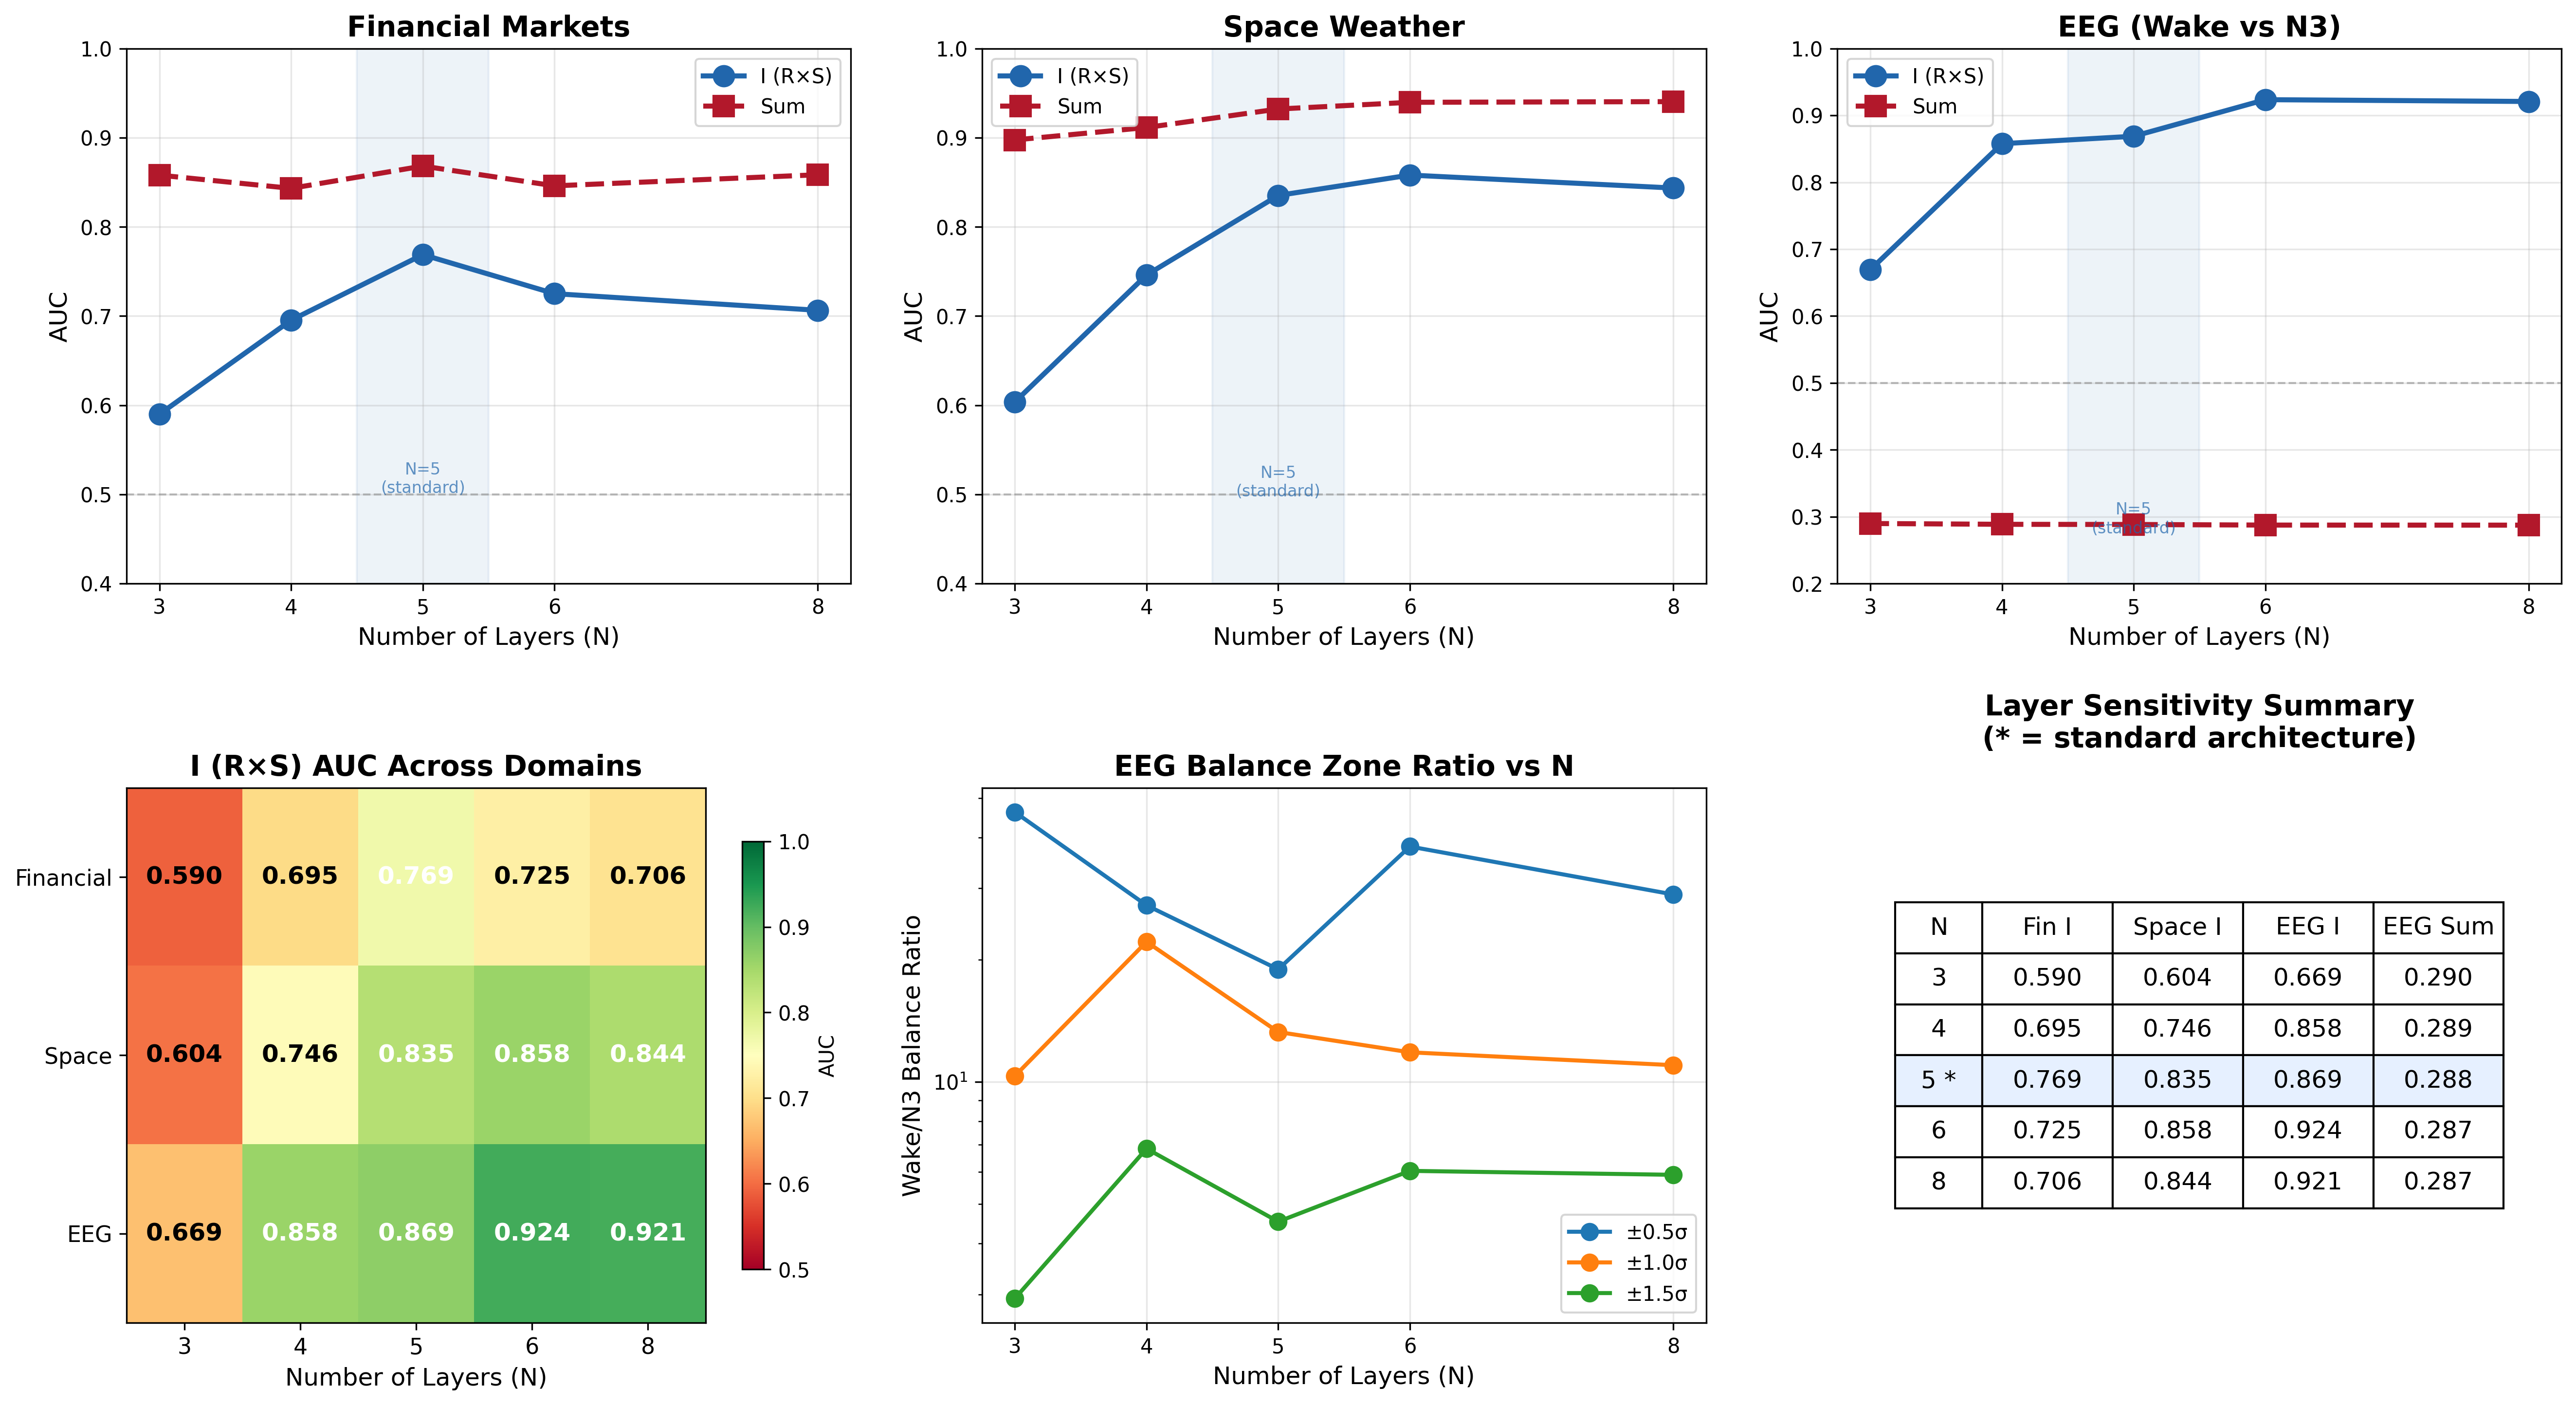
\includegraphics[width=\textwidth]{fig6_layer_sensitivity.png}
\caption[AUC stability across layer counts N equals 3 to 8 for financial, space weather, and EEG domains]{\label{fig:layer_sensitivity}AUC stability across layer counts $N = 3$ to $N = 8$ for all three domains. The framework is robust to layer count, with performance degrading smoothly only at $N = 3$ (insufficient hierarchical depth). Sum continues to anti-predict in EEG at all layer counts.}
\end{figure*}

The EEG result at $N = 6$ (AUC 0.924) suggests that splitting delta into slow and fast sub-bands captures additional structure relevant to coherence-state discrimination, consistent with the known physiological distinction between delta-1 (0.5--2~Hz) and delta-2 (2--4~Hz) oscillations~\cite{amzica1998}. However, we retain the five-layer architecture as the standard to maintain the zero-tuning claim---selecting $N = 6$ specifically for EEG would constitute domain-specific optimization.


\section{Discussion}

\subsection{The $I$--$D$ Balance as a Dynamic Existence Threshold}

The results across three domains support a consistent interpretation: the $I$--$D$ balance zone constitutes a dynamic existence threshold for organized system states. Systems in the balance zone---where integration and differentiation are jointly sustained---exhibit the hallmarks of healthy function: financial markets operate normally, the magnetosphere is in its quiet-time configuration, and the brain is awake and processing information. Departures from the balance zone correspond to qualitatively different states: cascading failures, geomagnetic storms, and the unconsciousness of deep sleep.

The directional dynamics analysis (Test~1) confirms that the system is constrained to the CASCADE--RECOVERY axis of the four-state model (Table~I). The CASCADE pattern (rising $I$, falling $D$) dominates during event periods, accounting for 45--51\% of event time steps. This pattern maps directly to the pathological synchronization observed in financial contagion~\cite{forbes2002}, geomagnetic storm development, and epileptic seizure propagation~\cite{lehnertz2009}. The near-absence of the COINCIDENCE pattern ($<$2\% during events) suggests a fundamental budget constraint: systems cannot simultaneously increase both integration and differentiation during critical periods.

A candidate mechanistic account follows from the general principle that coordination (synergy) is more fragile than overlap (redundancy) under system perturbation. As a system approaches a critical transition, the effective dimensionality of information transfer decreases. This compression preferentially destroys synergy (the $S$ component of $I = R \times S$), such that integration collapses while redundancy (and thus differentiation) may remain elevated. Under this account, the system moves from the balance zone into the cascade quadrant not by a symmetric process but by the asymmetric fragility of synergy---a pattern consistent with both information-theoretic expectations and the directional dynamics data presented here.

The strong $I$--$D$ anticorrelation ($\rho = -0.985$ in EEG; Section~3.6.4) means that the proxy metrics operate on a near-one-dimensional manifold parameterized by multi-scale entropy. The four-state model (Table~I) is a theoretical taxonomy of the full $I$--$D$ plane, not a description of the region accessible with these proxies. CASCADE and RECOVERY dominate empirically because they correspond to movement along the entropy axis; COINCIDENCE and COLLAPSE are rare because they require orthogonal movement that entropy-coupled metrics cannot produce. Future work with entropy-decoupled metrics---partial information decomposition~\cite{williams2010}, network mutual information, or graph-theoretic topology measures---could test whether the full two-dimensional $I$--$D$ plane is accessible when integration and differentiation are measured independently. For now, the framework is most accurately described as a multi-scale entropy coordinate system in which critical transitions manifest as rapid, high-variance departures from baseline entropy.

\subsection{Critical Slowing Down in $I$--$D$ Coordinates}

The early warning signal (Test~3)---rising variance of $|I - D|$ before events---connects the DET framework directly to the well-established critical transitions literature~\cite{scheffer2009,dakos2012}. Critical slowing down predicts that as a system approaches a bifurcation point, its recovery rate from perturbations decreases, leading to increasing variance and autocorrelation in state variables. The $I$--$D$ balance metric provides a natural coordinate in which to measure this phenomenon: the system's ability to maintain balance degrades as it approaches the transition, producing larger and larger fluctuations in $|I - D|$.

The quantitative consistency across domains---a 2.0$\times$ variance elevation at 5-day lead in both financial and space weather data---is noteworthy. While the temporal scales of the underlying processes differ (financial cascades build over weeks, geomagnetic storms over days), the early warning signal has similar magnitude at similar lead times. This suggests that the $I$--$D$ coordinate system may capture a domain-general feature of approaching transitions, though the author cautions against over-interpreting numerical coincidences from two domains.

The decay profile of the early warning signal differs between domains in a physically sensible way. Financial markets show persistent elevation out to 30 days, consistent with the slow build-up of systemic stress through leverage accumulation and correlation tightening. Space weather shows rapid decay by 15 days, consistent with the faster dynamics of solar wind--magnetosphere coupling. An $I$--$D$ framework that showed identical decay profiles across domains would be suspicious; the observed domain-appropriate decay profiles increase confidence that the framework is capturing genuine physics rather than statistical artifacts.

\subsection{Why Sum Fails: Structure Versus Magnitude}

The EEG results provide the strongest evidence for the DET framework's construct validity. The Sum anti-prediction (AUC 0.288--0.416) is not merely a failure---it is an \emph{informative} failure that illuminates what the framework measures.

Consider two hypothetical explanations for why $I$--$D$ balance discriminates system states:

\begin{enumerate}
\item \textbf{Magnitude hypothesis:} Events and state changes are simply associated with higher (or lower) total activity, and the $I$--$D$ framework captures this through its integration metric.
\item \textbf{Structure hypothesis:} Events and state changes are associated with changes in the \emph{organizational structure} of multi-component coupling, which is partially but imperfectly correlated with total activity.
\end{enumerate}

In financial markets and space weather, these hypotheses make similar predictions: cascades involve elevated activity across most layers, so both Sum and $I$ should discriminate. The data are consistent with both hypotheses in these domains (Sum AUC 0.868--0.932, $I$-based AUC 0.692--0.843).

The EEG domain dissociates the two hypotheses. N3 deep sleep has \emph{higher} total spectral power than wakefulness (massive delta oscillations), so the magnitude hypothesis predicts that Sum should classify N3 as the ``event'' state---which is indeed what happens, producing the anti-prediction. The structure hypothesis predicts that $I$ ($R \times S$) should correctly identify wakefulness as the state with higher integration, because wake involves coordinated multi-band activity while N3 involves single-band dominance---which is also what happens (AUC 0.869--0.904).

The dissociation is clean, the effect is large, and it scales with sample size. This constitutes strong evidence that the $I$--$D$ framework captures organizational structure rather than mere magnitude, validating the construct at the heart of the Dynamic Existence Threshold.

A natural question is whether domain-specific spectral ratios---particularly the delta/beta power ratio, a standard sleep staging feature---outperform $R \times S$ on the EEG task. Head-to-head comparison on the same 50-subject cohort yields delta/beta AUC $= 0.912$ vs.\ $R \times S$ AUC $= 0.901$ (bootstrap 95\% CI for the difference: [$-$0.013, $-$0.008], $p < 0.05$). The two metrics are highly correlated (Spearman $\rho = 0.923$), confirming that $R \times S$ partially recapitulates spectral power distribution information. However, on harder discrimination tasks---N1 vs.\ N2 ($R \times S$ AUC 0.740 vs.\ delta/beta 0.685) and Wake vs.\ N2 (0.532 vs.\ 0.502)---$R \times S$ outperforms the spectral ratio, suggesting that the multi-band integration measure captures organizational structure that a two-band ratio misses. Crucially, the delta/beta ratio is undefined outside neuroscience: financial markets and space weather have no frequency bands. The DET framework's contribution is not that $R \times S$ is the optimal classifier for any single domain, but that it provides a substrate-independent coordinate system in which state transitions are interpretable across all three domains tested---including the one where a domain-specific shortcut exists.

\subsection{Cross-Domain Consistency and the Limits of Broad Generality}

The results demonstrate broad generality of the DET framework across three substrates (socioeconomic, geophysical, biological) without parameter tuning. However, the author is careful to distinguish between two claims:

\begin{enumerate}
\item \textbf{Narrow claim (supported):} The $I$--$D$ balance framework provides a useful coordinate system for characterizing critical transitions across multiple domains, and its predictions are confirmed in all three domains tested.
\item \textbf{Strong claim (not yet supported):} The $I$--$D$ balance framework captures a universal principle that applies to all complex systems undergoing critical transitions.
\end{enumerate}

The narrow claim is well-supported by the data. The strong claim would require testing across a much wider range of systems---ecological tipping points, cellular state transitions, social network cascades, engineered system failures---and would need to account for systems where the five-layer decomposition may not have a natural interpretation.

The cross-domain transfer results (Test~4) illustrate both the promise and the limitations of broad generality. Sum-based thresholds transfer reasonably between financial and space weather domains (1.47$\times$ ratio, 0.78 TPR), but $R \times S$ thresholds diverge more (3.77$\times$ ratio). This suggests that while the \emph{qualitative} structure of $I$--$D$ space is domain-general, the \emph{quantitative} calibration of integration metrics is domain-specific. The $z$-score normalization of the balance metric partially addresses this by converting domain-specific scales to comparable units, but it does not fully eliminate the issue.

\subsection{Relation to Existing Frameworks}

The DET framework intersects with several established theoretical traditions.

\textbf{Integrated Information Theory}~\cite{tononi2016}. IIT's $\Phi$ quantifies integrated information as the information generated by a system above and beyond its parts. The DET framework draws inspiration from IIT's emphasis on integration but differs in two ways: (a) it adds an explicit differentiation coordinate, creating a two-dimensional state space rather than a single scalar; and (b) it uses empirically tractable proxy metrics ($R \times S$ for integration, JSD for differentiation) rather than computing $\Phi$ directly, which remains intractable for systems of even moderate size. The four-state model can be seen as a coarse-graining of the $I$--$D$ plane that may correspond heuristically to regimes of high and low $\Phi$, though $R \times S$ is a computationally tractable proxy rather than a formal information-theoretic measure of integrated information.

\textbf{Critical transitions theory}~\cite{scheffer2009,strogatz2015}. The DET framework provides a specific coordinate system ($I$--$D$ space) and a specific indicator (variance of $B = |z(I) - z(D)|$) for the general phenomenon of critical slowing down. This is complementary to existing approaches that use variance and autocorrelation of raw state variables~\cite{dakos2012}. The $I$--$D$ coordinate system has the advantage of being explicitly multi-scale (through the five-layer architecture) and of separating structural organization from magnitude.

\textbf{Perturbational complexity}~\cite{casali2013,sarasso2015}. The perturbational complexity index (PCI) measures the information content of the brain's response to transcranial magnetic stimulation, and has been shown to discriminate conscious from unconscious states. PCI is high when the response is both integrated (spatially widespread) and differentiated (temporally complex)---precisely the conditions that define the balance zone in the DET framework. The EEG results reported here are consistent with PCI findings, achieved through passive observation rather than perturbation.

\textbf{Self-organized criticality (SOC)}~\cite{bak1987,olami1992,strogatz2015}. The balance zone may correspond to the critical state in SOC models---the state to which the system self-organizes and from which avalanches (events) depart. The residence time results (Test~2) are consistent with this interpretation: the system spends more time in the balance zone during normal periods, as expected if the balance zone is an attractor, and exits rapidly during events, as expected if events are excursions from the critical state.

\textbf{Partial information decomposition (PID)}~\cite{williams2010,aguilera2019,popiel2020}. The $R$ and $S$ metrics are inspired by but not identical to the redundancy and synergy of PID. PID provides exact decompositions of mutual information into redundant, synergistic, and unique components; $R$ and $S$ are empirical proxies designed for tractability across domains. A formal connection between the DET framework's $R \times S$ and PID's synergy would strengthen the theoretical foundations of this work.

\subsection{Limitations}

Several limitations warrant explicit acknowledgment.

\textbf{Five-layer architecture.} The choice of exactly five layers is pragmatic rather than principled. However, the layer sensitivity analysis (Section~3.7, Table~\ref{tab:layers_sensitivity}) demonstrates that the framework is robust to this choice: adjacent layer counts ($N = 4$ and $N = 6$) produce AUC within 10\% of the $N = 5$ baseline across all three domains, with $N = 6$ actually improving performance in EEG (0.924 vs.\ 0.869) and space weather (0.858 vs.\ 0.835). The five-layer count is not a local optimum but a pragmatic choice within a broad robustness plateau spanning $N = 4$ to $N = 8$. Performance degrades only at $N = 3$, where insufficient hierarchical depth limits integration measurement.

\textbf{Proxy metrics and entropy coupling.} $R \times S$ and JSD are proxies for integration and differentiation, not exact information-theoretic quantities. Critically, both are functions of the Shannon entropy $H$ of the layer distribution: $R$ is derived from $N_{\text{eff}} = \exp(H)$ and increases with $H$, while $D = \text{JSD}^{1/2}(\mathbf{p} \| \mathbf{u})$ decreases with $H$ as the distribution approaches uniformity. This entropy coupling produces a Spearman anticorrelation of $\rho = -0.985$ in EEG (Section~3.6.4), constraining the nominally two-dimensional $I$--$D$ space to a near-one-dimensional manifold. Two of the four theoretical states (Organized complexity: high $I$, high $D$; Death/off: low $I$, low $D$) are rendered empirically inaccessible because they require $I$ and $D$ to covary rather than anti-covary. Under near-perfect anticorrelation, the balance metric $B = |z(I) - z(D)|$ reduces to approximately $|2\,z(I)|$---the absolute deviation of entropy from its historical mean. Entropy-decoupled measures---such as network mutual information, PID synergy~\cite{williams2010}, or graph-theoretic connectivity---might yield a genuinely two-dimensional $I$--$D$ space in which all four states are accessible. The empirical findings reported here (cross-domain transfer, early warning signals, structure-versus-magnitude dissociation) do not depend on the dimensionality claim and hold on the entropy axis alone.

\textbf{Temporal resolution.} Financial and space weather data are analyzed at daily resolution, while EEG is analyzed at 30-second epoch resolution. The framework has not been tested at intermediate timescales or at the sub-second resolution relevant to neural dynamics. The balance zone dynamics might differ qualitatively at different temporal scales.

\textbf{Event definition.} The definition of ``events'' in each domain relies on established criteria (VIX thresholds, Dst thresholds, sleep stage scoring), but these criteria are themselves imperfect. The framework's performance could be sensitive to event definition, particularly for boundary cases.

\textbf{Sample size in EEG.} The current results are based on 50 subjects (57,212 epochs). While the signal strengthens monotonically from 5 to 50 subjects (Table~\ref{tab:eeg}), the sample remains modest by neuroimaging standards. Replication in larger and more diverse cohorts is needed.

\textbf{Causal ambiguity.} The framework demonstrates that $I$--$D$ balance \emph{discriminates} system states and that its variance provides \emph{early warning} of transitions, but it does not establish that $I$--$D$ imbalance \emph{causes} transitions. The relationship could be correlational, with both $I$--$D$ dynamics and transitions driven by a common underlying process.

\textbf{Domain selection.} Three domains, while spanning physical, biological, and socioeconomic systems, constitute a limited sample. Domains were selected in part because they have well-defined ``event'' periods and accessible multi-layer data---a convenience sample that may not be representative of complex systems in general.


\section{Conclusion}

This paper introduced the Dynamic Existence Threshold---the hypothesis that systems persist in the zone where integration and differentiation are jointly sustained, and that critical events correspond to departures from this zone. Five quantitative tests, validated by permutation-based negative controls and comparison with standard early warning indicators, across three domains (financial markets, space weather, and human EEG) support this hypothesis:

\begin{enumerate}
\item Events cluster at $I$--$D$ extremes while normal states occupy the balance center, with the CASCADE pattern (rising $I$, falling $D$) accounting for 45--51\% of event dynamics.
\item Events exit the balance zone faster than normal state changes, with residence times halved during event periods ($p = 0.0001$ in financial data).
\item Rising variance of the balance metric $B = |z(I) - z(D)|$ provides early warning 5--30 days before events, with a 2.0$\times$ elevation ratio observed independently in both financial and space weather domains.
\item Exit velocity discriminates events from normal states with AUC 0.692--0.843, and cross-domain threshold transfer achieves 0.78 TPR without recalibration.
\item In EEG, the coupling structure metric $R \times S$ achieves AUC 0.909 (95\% CI [0.904, 0.913]) for discriminating wakefulness from deep sleep, while the simple sum anti-predicts (AUC 0.288--0.416), confirming that the framework captures organizational structure rather than magnitude.
\end{enumerate}

These results extend integrated information theory and critical transitions research into a dynamic framework that characterizes not just whether a system can persist as an organized entity, but the conditions under which it transitions between qualitatively different states. The $I$--$D$ balance zone emerges as a broadly general feature of complex systems, providing a common coordinate system for understanding critical transitions across substrates.

The practical implication is a domain-general early warning indicator: rising variance of the balance metric $B$, computed from any system that can be decomposed into multiple measurement layers. The theoretical implication is that the multi-scale entropy captured by the integration--differentiation decomposition provides a coordinate system in which the approach to critical transitions is measurable, with the balance zone corresponding to entropy near its historical baseline and departures signaling organizational state change.


\section*{Supplementary Material}

See supplementary material for complete analysis code, pre-computed results, and publication figures at \url{https://github.com/existencethreshold/dynamic-existence-threshold}.

\section*{Acknowledgments}
The framework emerged from practical work on distributed system monitoring, which motivated the integration-differentiation decomposition.

\emph{AI tools acknowledgment:} AI tools (Claude, Gemini) were used to assist with code generation, statistical analysis, and manuscript revision. All scientific claims, interpretations, and editorial decisions are the sole responsibility of the author.

\section*{Author Declarations}

\noindent\textbf{Conflict of Interest:} The author has no conflicts to disclose.
\medskip

\noindent\textbf{Ethics Approval:} This study analyzed publicly available, de-identified datasets. The EEG data are from the Sleep-EDF dataset hosted on PhysioNet; ethical approval for the original data collection was obtained from the dataset creators (Kemp et al., 2000).
\medskip

\noindent\textbf{Author Contributions (CRediT):} Nathan M. Thornhill: Conceptualization (lead); Data curation (lead); Formal analysis (lead); Investigation (lead); Methodology (lead); Software (lead); Validation (lead); Visualization (lead); Writing -- original draft (lead); Writing -- review \& editing (lead).

\section*{Data Availability Statement}

The data that support the findings of this study are openly available. Financial data are derived from publicly available market indices via the yfinance Python library. Space weather data are from NASA OMNI2 (\url{https://omniweb.gsfc.nasa.gov/}). EEG data are from the Sleep-EDF dataset on PhysioNet (\url{https://physionet.org/content/sleep-edfx/}). Complete analysis code and pre-computed results are available at \url{https://github.com/existencethreshold/dynamic-existence-threshold}.

\begin{thebibliography}{33}

\bibitem{scheffer2009} M. Scheffer, J. Bascompte, W. A. Brock, V. Brovkin, S. R. Carpenter, V. Dakos, H. Held, E. H. van Nes, M. Rietkerk, and G. Sugihara, ``Early-warning signals for critical transitions,'' Nature \textbf{461}(7260), 53--59 (2009).

\bibitem{dakos2012} V. Dakos, S. R. Carpenter, W. A. Brock, A. M. Ellison, V. Guttal, A. R. Ives, S. K{\'e}fi, V. Livina, D. A. Seekell, E. H. van Nes, and M. Scheffer, ``Methods for detecting early warnings of critical transitions in time series illustrated using simulated ecological data,'' PLoS ONE \textbf{7}(7), e41010 (2012).

\bibitem{tononi2016} G. Tononi, M. Boly, M. Massimini, and C. Koch, ``Integrated information theory: From consciousness to its physical substrate,'' Nat. Rev. Neurosci. \textbf{17}(7), 450--461 (2016).

\bibitem{tononi2004} G. Tononi, ``An information integration theory of consciousness,'' BMC Neurosci. \textbf{5}, 42 (2004).

\bibitem{baars1988} B. J. Baars, \emph{A Cognitive Theory of Consciousness} (Cambridge University Press, 1988).

\bibitem{seth2011} A. K. Seth, A. B. Barrett, and L. Barnett, ``Causal density and integrated information as measures of conscious level,'' Philos. Trans. R. Soc. A \textbf{369}(1952), 3748--3767 (2011).

\bibitem{berry2017} R. B. Berry, R. Brooks, C. E. Gamaldo, S. M. Harding, R. M. Lloyd, C. L. Marcus, and B. V. Vaughn, ``The AASM manual for the scoring of sleep and associated events: Rules, terminology and technical specifications, version 2.4,'' American Academy of Sleep Medicine (2017).

\bibitem{oppenheim1997} A. V. Oppenheim and A. S. Willsky, \emph{Signals and Systems}, 2nd ed. (Prentice Hall, 1997).

\bibitem{muthukumaraswamy2013} S. D. Muthukumaraswamy, ``High-frequency brain activity and muscle artifacts in MEG/EEG: A review and recommendations,'' Front. Hum. Neurosci. \textbf{7}, 138 (2013).

\bibitem{papitashvili2020} N. E. Papitashvili and J. H. King, ``OMNI hourly data set,'' NASA Space Physics Data Facility (2020). \url{https://omniweb.gsfc.nasa.gov/}

\bibitem{forbes2002} K. J. Forbes and R. Rigobon, ``No contagion, only interdependence: Measuring stock market comovements,'' J. Finance \textbf{57}(5), 2223--2261 (2002).

\bibitem{hill1973} M. O. Hill, ``Diversity and evenness: A unifying notation and its consequences,'' Ecology \textbf{54}(2), 427--432 (1973).

\bibitem{jost2006} L. Jost, ``Entropy and diversity,'' Oikos \textbf{113}(2), 363--375 (2006).

\bibitem{pielou1966} E. C. Pielou, ``The measurement of diversity in different types of biological collections,'' J. Theor. Biol. \textbf{13}, 131--144 (1966).

\bibitem{lin1991} J. Lin, ``Divergence measures based on the Shannon entropy,'' IEEE Trans. Inf. Theory \textbf{37}(1), 145--151 (1991).

\bibitem{endres2003} D. M. Endres and J. E. Schindelin, ``A new metric for probability distributions,'' IEEE Trans. Inf. Theory \textbf{49}(7), 1858--1860 (2003).

\bibitem{gonzalez1994} W. D. Gonzalez, J. A. Joselyn, Y. Kamide, H. W. Kroehl, G. Rostoker, B. T. Tsurutani, and V. M. Vasyliunas, ``What is a geomagnetic storm?'' J. Geophys. Res. \textbf{99}(A4), 5771--5792 (1994).

\bibitem{kemp2000} B. Kemp, A. H. Zwinderman, B. Tuk, H. A. C. Kamphuisen, and J. J. L. Obery{\'e}, ``Analysis of a sleep-dependent neuronal feedback loop: The sleep-EDF database,'' IEEE Trans. Biomed. Eng. \textbf{47}(9), 1185--1194 (2000).

\bibitem{goldberger2000} A. L. Goldberger, L. A. N. Amaral, L. Glass, J. M. Hausdorff, P. Ch. Ivanov, R. G. Mark, J. E. Mietus, G. B. Moody, C.-K. Peng, and H. E. Stanley, ``PhysioBank, PhysioToolkit, and PhysioNet: Components of a new research resource for complex physiologic signals,'' Circulation \textbf{101}(23), e215--e220 (2000).

\bibitem{benjamini1995} Y. Benjamini and Y. Hochberg, ``Controlling the false discovery rate: A practical and powerful approach to multiple testing,'' J. R. Stat. Soc. Ser. B \textbf{57}(1), 289--300 (1995).

\bibitem{massimini2005} M. Massimini, F. Ferrarelli, R. Huber, S. K. Esser, H. Singh, and G. Tononi, ``Breakdown of cortical effective connectivity during sleep,'' Science \textbf{309}(5744), 2228--2232 (2005).

\bibitem{niedermeyer2005} E. Niedermeyer and F. L. da Silva, \emph{Electroencephalography: Basic Principles, Clinical Applications, and Related Fields}, 5th ed. (Lippincott Williams \& Wilkins, 2005).

\bibitem{buzsaki2006} G. Buzs{\'a}ki, \emph{Rhythms of the Brain} (Oxford University Press, 2006).

\bibitem{casali2013} A. G. Casali, O. Gosseries, M. Rosanova, M. Boly, S. Sarasso, K. R. Casali, S. Casarotto, M.-A. Bruno, S. Laureys, G. Tononi, and M. Massimini, ``A theoretically based index of consciousness independent of sensory processing and behavior,'' Sci. Transl. Med. \textbf{5}(198), 198ra105 (2013).

\bibitem{amzica1998} F. Amzica and M. Steriade, ``Electrophysiological correlates of sleep delta waves,'' Electroencephalogr. Clin. Neurophysiol. \textbf{107}(2), 69--83 (1998).

\bibitem{lehnertz2009} K. Lehnertz, S. Bialonski, M.-T. Horstmann, D. Krug, A. Rothkegel, M. Staniek, and T. Wagner, ``Synchronization phenomena in human epileptic brain networks,'' J. Neurosci. Methods \textbf{183}(1), 42--48 (2009).

\bibitem{strogatz2015} S. H. Strogatz, \emph{Nonlinear Dynamics and Chaos}, 2nd ed. (Westview Press, 2015).

\bibitem{sarasso2015} S. Sarasso, M. Boly, M. Napolitani, O. Gosseries, V. Charland-Verville, S. Casarotto, M. Rosanova, A. G. Casali, J.-F. Brichant, P. Boveroux, S. Rex, G. Tononi, S. Laureys, and M. Massimini, ``Consciousness and complexity during unresponsiveness induced by propofol, xenon, and ketamine,'' Curr. Biol. \textbf{25}(23), 3099--3105 (2015).

\bibitem{bak1987} P. Bak, C. Tang, and K. Wiesenfeld, ``Self-organized criticality: An explanation of $1/f$ noise,'' Phys. Rev. Lett. \textbf{59}(4), 381--384 (1987).

\bibitem{olami1992} Z. Olami, H. J. S. Feder, and K. Christensen, ``Self-organized criticality in a continuous, nonconservative cellular automaton modeling earthquakes,'' Phys. Rev. Lett. \textbf{68}(8), 1244--1247 (1992).

\bibitem{williams2010} P. L. Williams and R. D. Beer, ``Nonnegative decomposition of multivariate information,'' arXiv:1004.2515 (2010).

\bibitem{aguilera2019} M. Aguilera, S. A. Moosavi, and H. Shimazaki, ``Information-theoretic complexity and the structure of large-scale neural systems,'' arXiv:1906.04035 (2019).

\bibitem{popiel2020} N. J. Popiel, S. Bhatt, M. Engstr{\"o}m, K. Lindgren, and J. T. Lizier, ``Partial information decomposition and the emergence of redundancy in complex systems,'' Phys. Rev. E \textbf{102}(3), 032110 (2020).

\end{thebibliography}

\end{document}
